\documentclass[a4paper,12pt]{report}
%\documentclass[aps,twocolumn,secnumarabic,balancelastpage,amsmath,amssymb,nofootinbib,floatfix]{revtex4-1}
\usepackage[utf8]{inputenc}
\usepackage[a4paper, total={6in, 8in}]{geometry}
\usepackage{graphicx}
\usepackage{mathrsfs}
\usepackage{amsmath}
\usepackage{amsfonts}
\usepackage{sidecap}
\usepackage{setspace}
\usepackage{fancyvrb}

\renewcommand{\thesection}{\arabic{section}}

\begin{document}

\title{Numerically Modeling Gravitationally Bound Systems}
\author{Noah Green \\ Michigan State University}
%\affiliation{Michigan State University}
\date{April 1, 2016}
\maketitle
\begin{abstract}
The RK4 and Verlet algorithms for calculating the solutions to ordinary differential equations are used here to calculate the orbits of various gravitationally bound systems resembling the solar system. It was found that the RK4 algorithm is more accurate, but the Verlet algorithm is easier to implement. Additionally, systems that have many bodies that move on different timescales become difficult to model, requiring many more time steps to accurately model objects moving on a short timescale (e.g. Mercury) than is necessary to accurately model objects moving on a long timescale (e.g. Pluto). This was remedied in a model solar system by treating the inner and outer solar systems separately, and ignoring the negligible effect of the gravitational force due to the first four planets on the outer four planets and Pluto.
\end{abstract}

\doublespacing
\section{Introduction}\label{sec:intro}
Modeling the gravitational force has many applications, from space travel to astronomy. I will discuss how to use the Runge-Kutta and Verlet algorithms to numerically calculate the motion of model solar systems due to classical gravitational interactions. In section \ref{sec:diffeq}, I cover the equations used to model gravitational interactions. In section \ref{sec:alg}, I discuss how these equations can be solved numerically. In section \ref{sec:ss}, I show these algorithms applied in different situations. Finally, in section \ref{sec:conclude}, I summarize the conclusions of this study.

\section{Differential Equations}\label{sec:diffeq}
The force due to gravity between two objects can be calculated using Newton's law of gravitation:

\begin{equation}\label{eq:gravitation}
 F_G = \frac{GMm}{r^2}
\end{equation}

where $G$ is the universal gravitational constant, $M$ and $m$ are the masses of the two object, and $r$ is the distance between them. Newton's second law, $F = ma$ gives us that

\begin{equation}\label{eq:nsl}
 \frac{d^2x}{dt^2} = \frac{F_{G,m,x}}{m}
\end{equation}

with similar equations for $y$ and $z$. In order to use the algorithms, these equations must be rewritten as a set of coupled first order ordinary differential equations. For a planet orbiting the sun, these equations are

\begin{equation}\label{eq:dvx}
   \frac{dv_x}{dt}=-\frac{GM_{\odot}}{r^3}x,
\end{equation}

\begin{equation}\label{eq:dx}
   \frac{dx}{dt}=v_x,
\end{equation}

for the $x$ coordinate, with similar equations for $y$ and $z$ coordinates.

\section{Algorithms}\label{sec:alg}

  Both the Verlet and Runge-Kutta methods are based on Taylor expanding the ODE for which we want to solve ( e.g. equations (\ref{eq:dvx}) and (\ref{eq:dx}) ), discretizing the function in question, then using some trick to step through the discrete solutions based on initial conditions. Their derivation can be found in references \cite{Landau:2008} and \cite{Dux:2016}. I will cover how they can be used algorithmically.

\subsection{RK4}
In addition to a Taylor expansion, the Runge-Kutta method also utilizes midpoint approximations of the integral of a differential equation. Hence, different orders of this approximation, using any number of midpoints, can be used to get varying degrees of accuracy. The RK4 method uses two midpoints and the endpoints of each discrete interval. For a first order differential equation $\frac{dy}{dx} = f(t,y)$, we have
\[
  k_1=hf(t_i,y_i) \hspace{0.5cm}   k_2=hf(t_i+h/2,y_i+k_1/2)
\]
\[
  k_3=hf(t_i+h/2,y_i+k_2/2)\hspace{0.5cm}   k_4=hf(t_i+h,y_i+k_3)
  \]
to get the next value in the discretized solution
\begin{equation}
  y_{i+1}=y_i +\frac{1}{6}\left( k_1 +2k_2+2k_3+k_4\right).
\end{equation}

Applying this to equations (\ref{eq:dvx}) and (\ref{eq:dx}), first note that the right side of equation 
(\ref{eq:dvx}) can be represented for a planet with mass $m$ as $F_x(r)/m$. First calculate $k_1$
\begin{equation}
 x: k_1 = hv_{i-1} \hspace{0.5cm} v: k_1 = hF_x(r_{i})/m.
\end{equation}
where $h$ is the discrete time step. For the positional $k_2$, $k_3$, and $k_4$, simply add $k_1/2$, $k_2/2$, or $k_3$ respectively to the $i^{th}$ position. The velocity $k_2$, $k_3$, and $k_4$ then come automatically by recalculating the force at the new position and multiplying it by $h/m$. The complete code that I used can be found in appendix \ref{app:rk4}, but the abridged version follows:

\singlespacing
\begin{Verbatim}[fontsize=\small]
   for( int i = 1; i <= _Ntime; i++ ){
    vector< vector< double > > k1, k2, k3; 
    for( unsigned int iPlanet = 0; iPlanet < GetN(); iPlanet++ ){
    
    ... Calculate k1, k2, k3, k4...
    
    	_vPlanets.at(iPlanet).SetX(_vPlanets.at(iPlanet).X(i-1)
				   +(k1.at(iPlanet).at(0)
				   +2.*k2.at(iPlanet).at(0)
				   +2.*k3.at(iPlanet).at(0)
				     +k4i.at(0))/6.,i);
	_vPlanets.at(iPlanet).SetY(_vPlanets.at(iPlanet).Y(i-1)
				   +(k1.at(iPlanet).at(1)
				   +2.*k2.at(iPlanet).at(1)
				   +2.*k3.at(iPlanet).at(1)
				     +k4i.at(1))/6.,i);
	_vPlanets.at(iPlanet).SetZ(_vPlanets.at(iPlanet).Z(i-1)
				   +(k1.at(iPlanet).at(2)
				   +2.*k2.at(iPlanet).at(2)
				   +2.*k3.at(iPlanet).at(2)
				     +k4i.at(2))/6.,i);
	_vPlanets.at(iPlanet).SetVx(_vPlanets.at(iPlanet).Vx(i-1)
				    +(k1.at(iPlanet).at(3)
				    +2.*k2.at(iPlanet).at(3)
				    +2.*k3.at(iPlanet).at(3)
				      +k4i.at(3))/6.,i);
	_vPlanets.at(iPlanet).SetVy(_vPlanets.at(iPlanet).Vy(i-1)
				    +(k1.at(iPlanet).at(4)
				    +2.*k2.at(iPlanet).at(4)
				    +2.*k3.at(iPlanet).at(4)
				      +k4i.at(4))/6.,i);
	_vPlanets.at(iPlanet).SetVz(_vPlanets.at(iPlanet).Vz(i-1)
				    +(k1.at(iPlanet).at(5)
				    +2.*k2.at(iPlanet).at(5)
				    +2.*k3.at(iPlanet).at(5)
				      +k4i.at(5))/6.,i);
      }
    }
  }
\end{Verbatim}

This algorithm is the more accurate of the two covered in this paper, with a global error of $O(h^4)$.
\doublespacing


\subsection{Verlet}

The velocity Verlet method is more straightforward, but goes like $O(h^3)$. The equations to find the next discrete solution value are as follows.
\begin{equation}
x_{i+1} = x_i+hv_i+\frac{h^2}{2}a_{i},
\end{equation}
and
\begin{equation}
v_{i+1} = v_i+\frac{h}{2}\left( a_{i+1}+a_{i}\right). 
\end{equation}
where $a$ denotes the acceleration. The trickiest part of this algorithm is that the position needs to be calculated first. This lets us get $a_{i+1}$ by calculating the force from the new position and dividing by the planet's mass. I implemented this algorithm in C++ as follows:

\begin{Verbatim}[fontsize=\small]
void SolarSystem::Verlet(){
  _solved = true;
  // make force variables in this scope so they persist through loops
  vector<double> Fx,Fy,Fz;
  vector<double> fx,fy,fz;
  double f_x,f_y,f_z;
  for( unsigned int fi = 0; fi < GetN(); fi++ ){
    TotalForce(fi,0,f_x,f_y,f_z);
    Fx.push_back(f_x);
    Fy.push_back(f_y);
    Fz.push_back(f_z);
    fx.push_back(f_x);
    fy.push_back(f_y);
    fz.push_back(f_z);
  }

  for( int i = 1; i <= _Ntime; i++){
    for( unsigned int iPlanet = 0; iPlanet < GetN(); iPlanet++ ){
      if(_vPlanets.at(iPlanet).Fixed()){
	_vPlanets.at(iPlanet).AddCoordinates(i*_step,
					     _vPlanets.at(iPlanet).X(i-1),
					     _vPlanets.at(iPlanet).Y(i-1),
					     _vPlanets.at(iPlanet).Z(i-1),
					     _vPlanets.at(iPlanet).Vx(i-1),
					     _vPlanets.at(iPlanet).Vy(i-1),
					     _vPlanets.at(iPlanet).Vz(i-1));  
      }
      else{
	// advance spatial coordinates by one time step
	// set velocity to zero for now
	fx.at(iPlanet) = Fx.at(iPlanet);
	fy.at(iPlanet) = Fy.at(iPlanet);
	fz.at(iPlanet) = Fz.at(iPlanet);
	_vPlanets.at(iPlanet).AddCoordinates(i*_step,
					     _vPlanets.at(iPlanet).X(i-1)+ 
					     _step*_vPlanets.at(iPlanet).Vx(i-1)+
					     _step*_step*fx.at(iPlanet)/(2.*_vPlanets.at(iPlanet).M()),
					     _vPlanets.at(iPlanet).Y(i-1)+
					     _step*_vPlanets.at(iPlanet).Vy(i-1)+
					     _step*_step*fy.at(iPlanet)/(2.*_vPlanets.at(iPlanet).M()),
					     _vPlanets.at(iPlanet).Z(i-1)+
					     _step*_vPlanets.at(iPlanet).Vz(i-1)+
					     _step*_step*fz.at(iPlanet)/(2.*_vPlanets.at(iPlanet).M()),
					     0.,0.,0.);
      }
    }
    for( unsigned int iPlanet = 0; iPlanet < GetN(); iPlanet++){
      if( !_vPlanets.at(iPlanet).Fixed() ){
	// calculate force using new position coordinates
	TotalForce(iPlanet,i,Fx.at(iPlanet),Fy.at(iPlanet),Fz.at(iPlanet));
	// advance velocity coordinates by one step
	_vPlanets.at(iPlanet).SetVx(_vPlanets.at(iPlanet).Vx(i-1)+
				    _step*(fx.at(iPlanet)+Fx.at(iPlanet))/(2.*_vPlanets.at(iPlanet).M()),i);
	_vPlanets.at(iPlanet).SetVy(_vPlanets.at(iPlanet).Vy(i-1)+
				    _step*(fy.at(iPlanet)+Fy.at(iPlanet))/(2.*_vPlanets.at(iPlanet).M()),i);
	_vPlanets.at(iPlanet).SetVz(_vPlanets.at(iPlanet).Vz(i-1)+
				    _step*(fz.at(iPlanet)+Fz.at(iPlanet))/(2.*_vPlanets.at(iPlanet).M()),i);
	
      }
    }
  }
}
\end{Verbatim}

Note that the equations are for the $x$ components of the position and velocity only. As can be seen in the code, the other coordinates can be found using analogous equations.

\section{The Solar System}\label{sec:ss}
Armed with these algorithms, I was able to model several different systems. The simplest case is the Earth-Sun system, ignoring the other planets, assuming the sun is stationary and the orbit of Earth is circular. In the next case, I determined the velocity needed for a planet starting at 1 AU from the sun to escape from the solar system. By adding the forces on each planet due to all other bodies component-wise, I am then able to move onto three and more bodied systems culminating with all major bodies of the solar system. Note that for all calculations, I used the units of solar masses ($M_\odot$) for mass, AU (mean distance from Earth to the Sun) for distance, and years for time. For easier comparison, I have placed many of the resulting plots in the appendix.

\subsection{Earth-Sun only}\label{ssec:esf}
Figures \ref{fig:ESRK4_position} and \ref{fig:ESVerlet_position} were calculated so that Earth has a circular orbit. In appendix \ref{app:esplots}, additional plots of the angular momentum and kinetic and potential energy of the system are included. 

 \begin{SCfigure}
 \centering
   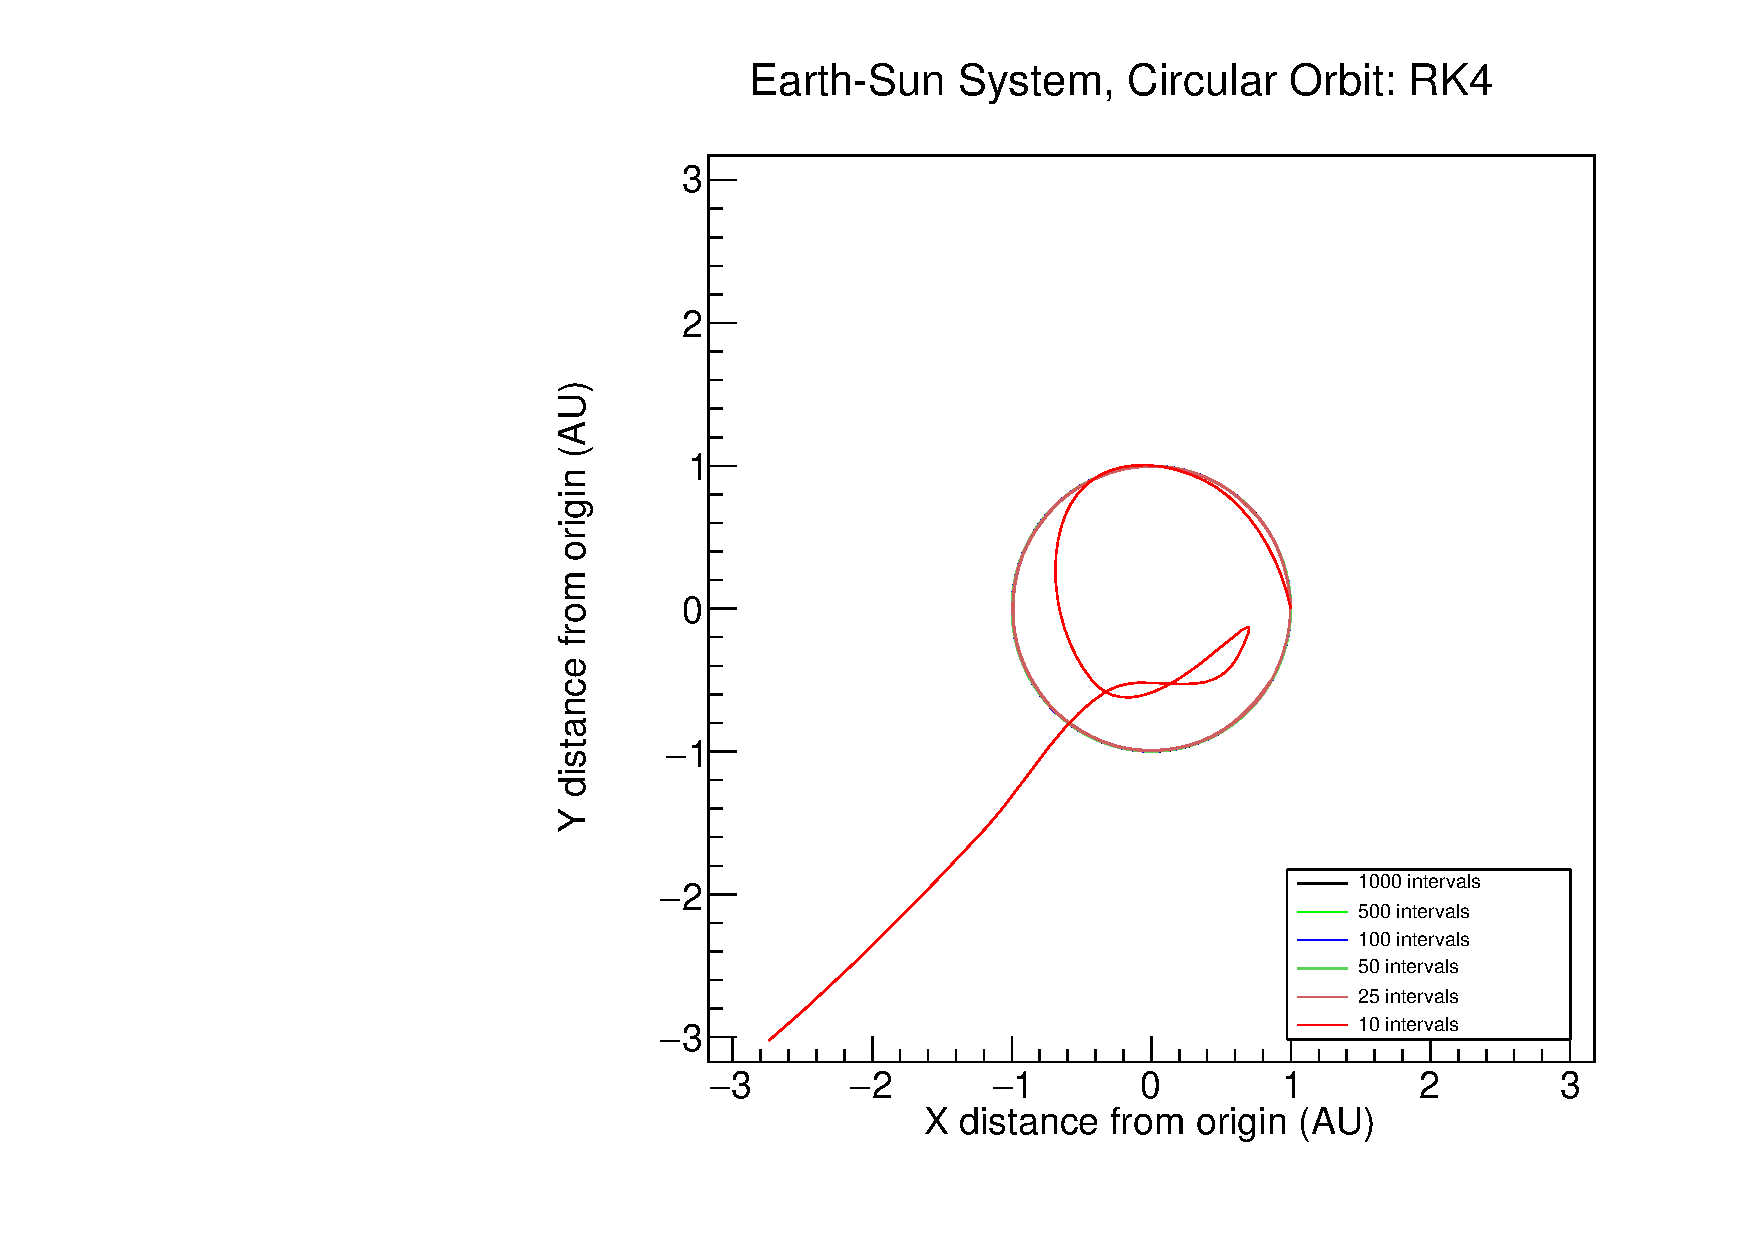
\includegraphics[width=0.5\textwidth]{ESRK4_position.pdf}
  \caption{Plot of Earth's position in Earth-Sun system for different numbers of time steps over 1.9 years using the RK4 algorithm.}
  \label{fig:ESRK4_position}
 \end{SCfigure}

  \begin{SCfigure}
 \centering
   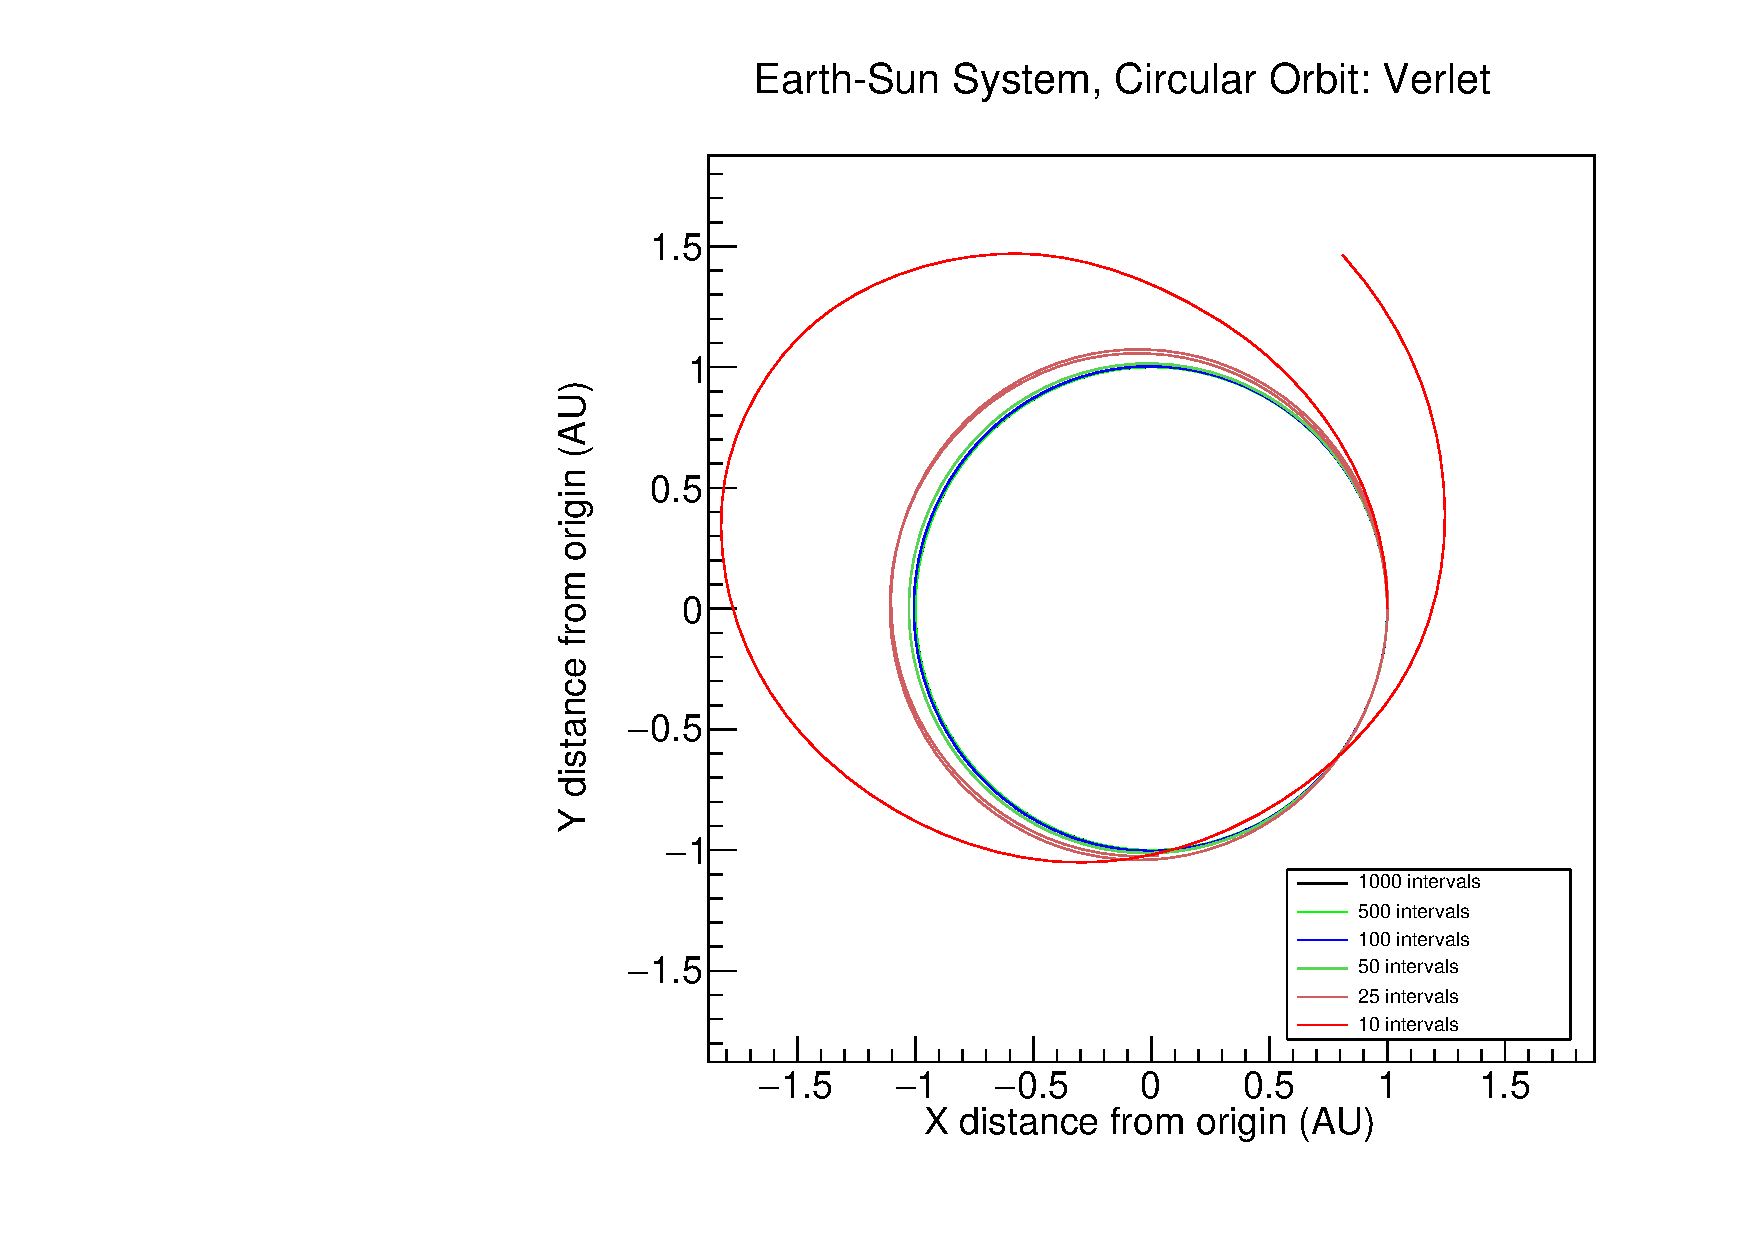
\includegraphics[width=0.5\textwidth]{ESVerlet_position.pdf}
  \caption{Plot of Earth's position in Earth-Sun system for different numbers of time steps over 1.9 years using the Verlet algorithm.}
  \label{fig:ESVerlet_position}
 \end{SCfigure}

 Note that the orbits in the Verlet plot of figure \ref{fig:ESVerlet_position} begin to noticeably diverge at 50 intervals, while the RK4 algorithm doesn't seem to diverge until somewhere between 10 and 25 intervals. Additionally, the kinetic energy, potential energy, and the angular momentum all converge to being constant at higher numbers of intervals. This is expected because a circular orbit has constant velocity and is at a constant distance from the sun.

\subsection{Escape Velocity}

Say that a planet with Earth's mass starts at 1 AU from a stationary sun. What velocity does it need in order to escape from the solar system? I found this out by noting that it needs enough kinetic energy to overcome the gravitational potential well of the sun. Hence, the escape velocity can be found by solving
\[
 \frac{1}{2}mv_{escape}^2-\frac{GM_\odot m}{r_0} = E = 0
\]
for the velocity $v_{escape}$. This gives us that the escape velocity is
\[
 v_{escape}=\sqrt{\frac{2GM_\odot}{r_0}}.
\]

 \begin{SCfigure}
 \centering
   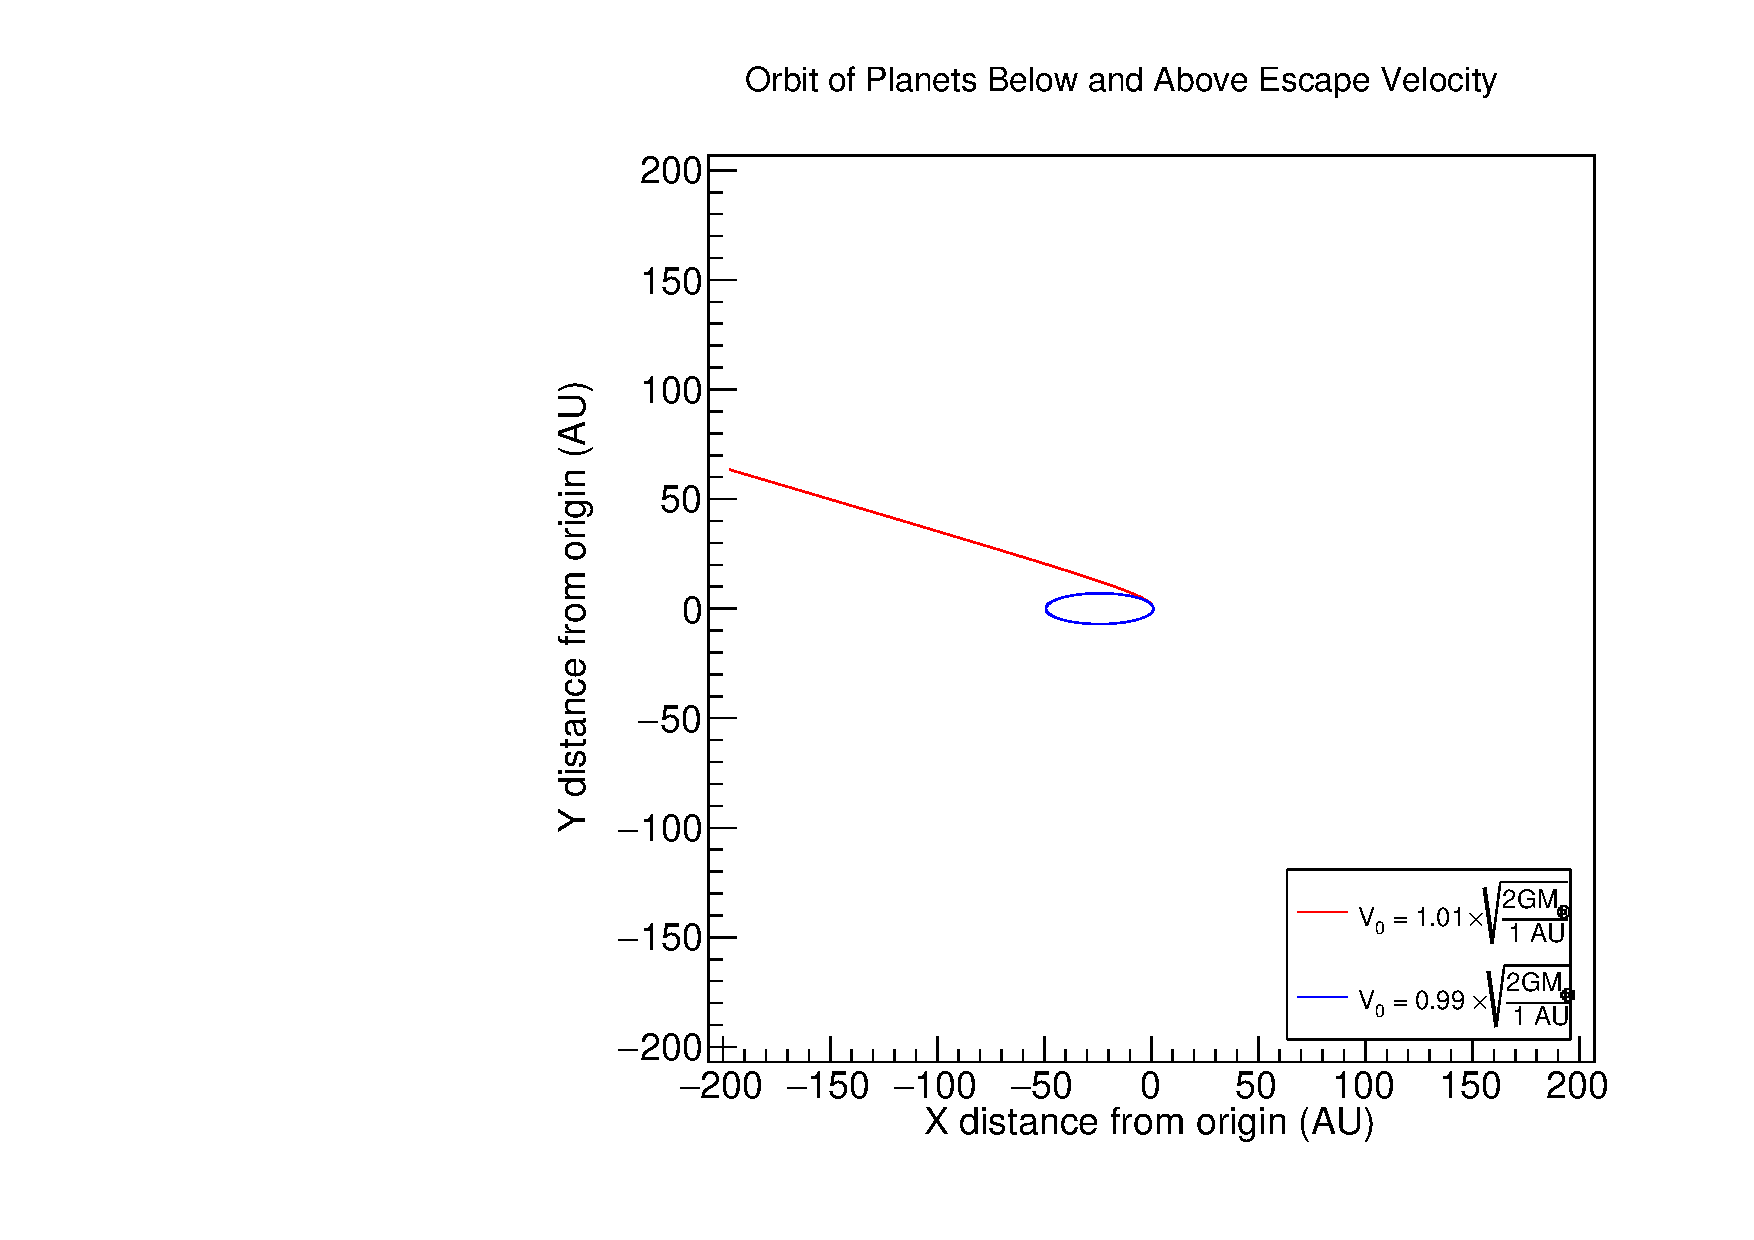
\includegraphics[width=0.5\textwidth]{Escape_plot.pdf}
  \caption{Plot of planet with starting position of 1 AU and starting mass of one Earth mass with initial velocity just above and below escape velocity. Orbital period found by trial and error to be 126 years for the planet just below escape velocity. 20000 time steps and the RK4 algorithm were used for accurate orbit modeling.}
  \label{fig:Escape}
 \end{SCfigure}

 Setting up a simulation of such a planet with velocity 1\% above and below the escape velocity, we can see in figure \ref{fig:Escape} that this derivation for the escape velocity is correct.
 
\subsection{Three Body System: Stationary Sun}\label{ssec:3bsss}
Equation (\ref{eq:gravitation}) applies to any two massive bodies. To get the total force on a planet, one must sum all of the forces from other massive bodies on the planet component-wise. The position and velocity of the planet may then be calculated in accordance with section \ref{sec:alg}. The movement of planets in a many body system can be calculated by finding the total force on each planet at each time step, and advancing their position all at the same time.

\begin{SCfigure}
 \centering
   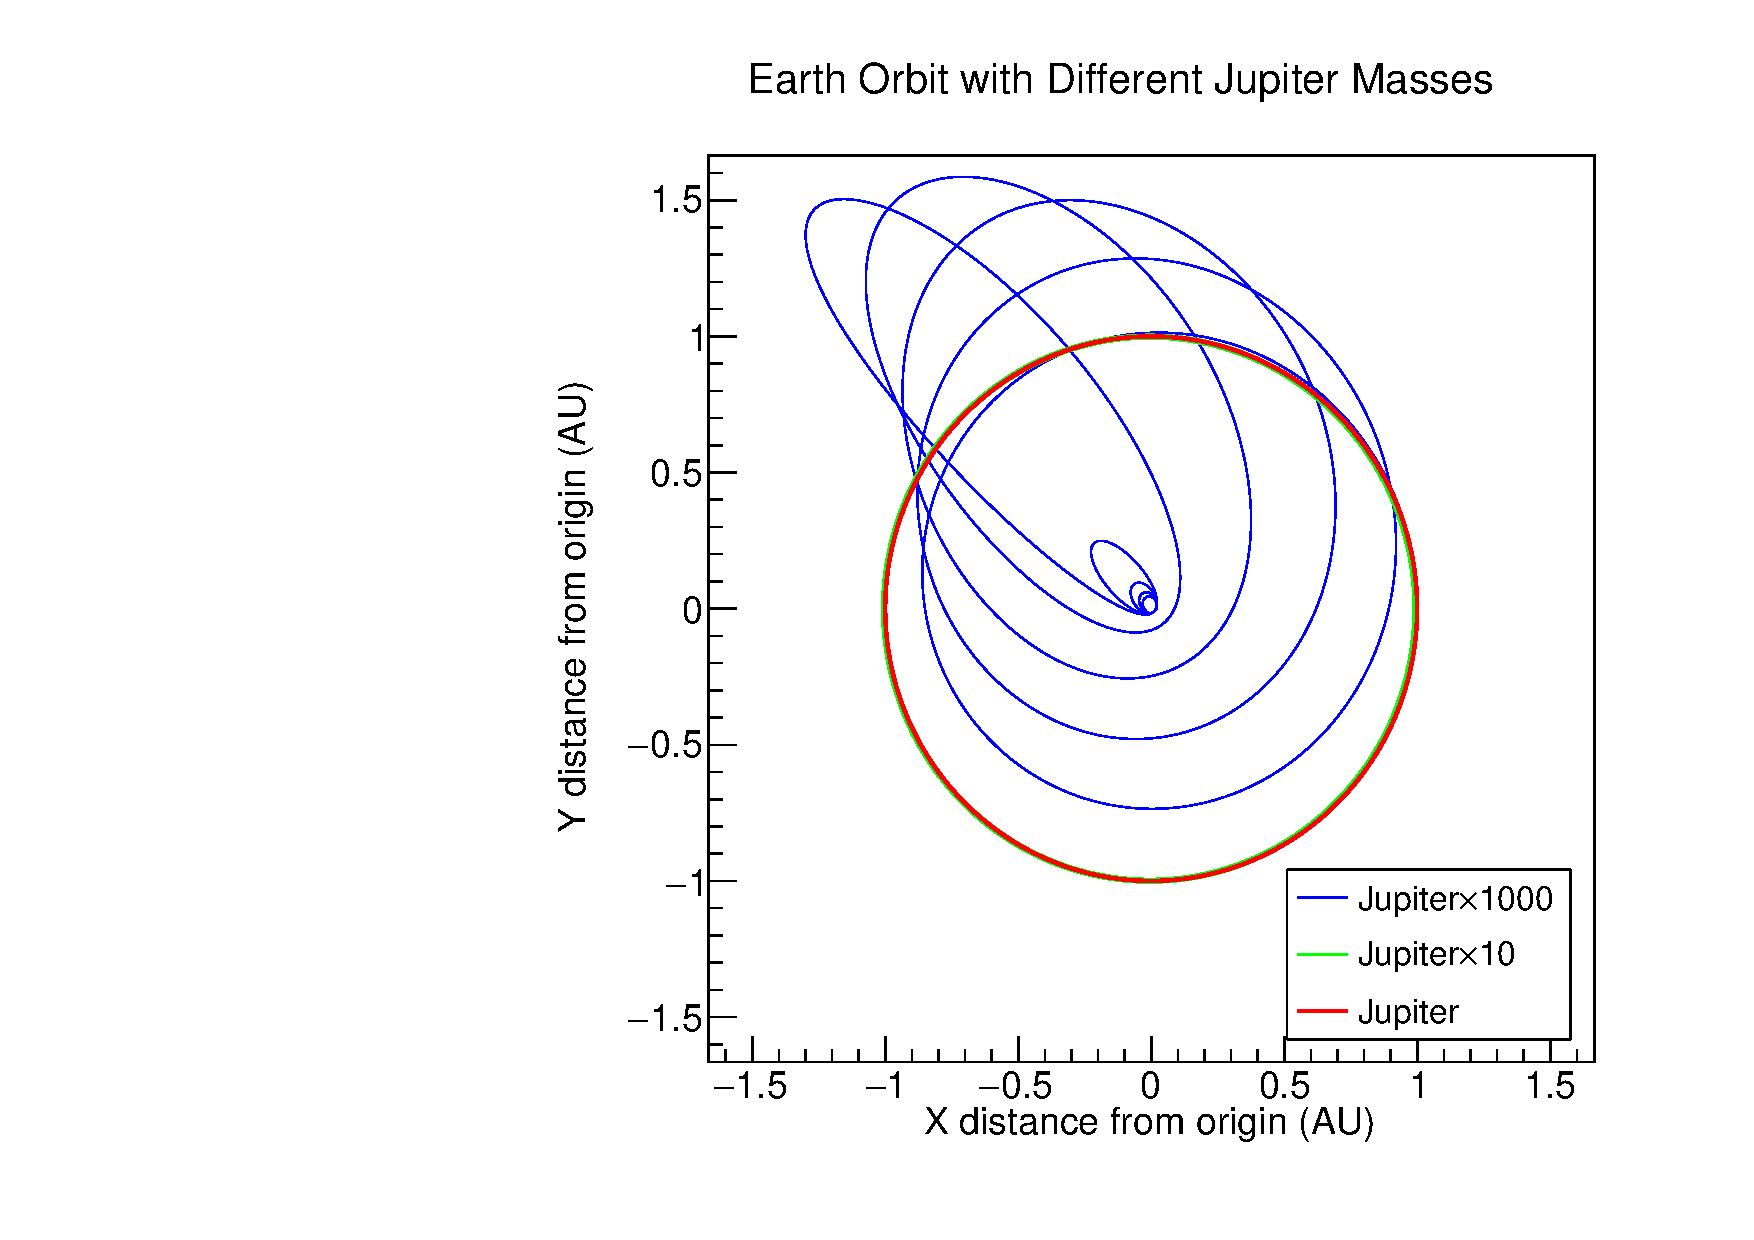
\includegraphics[width=0.5\textwidth]{ESJFRK4_Earths.pdf}
  \caption{Plot of the position of earth in three body system with stationary sun and different Jupiter masses. Used a time length of 13 years with 13000 time steps with the RK4 algorithm.}
  \label{fig:ESJFRK4_Earths}
 \end{SCfigure}

 \begin{SCfigure}
 \centering
   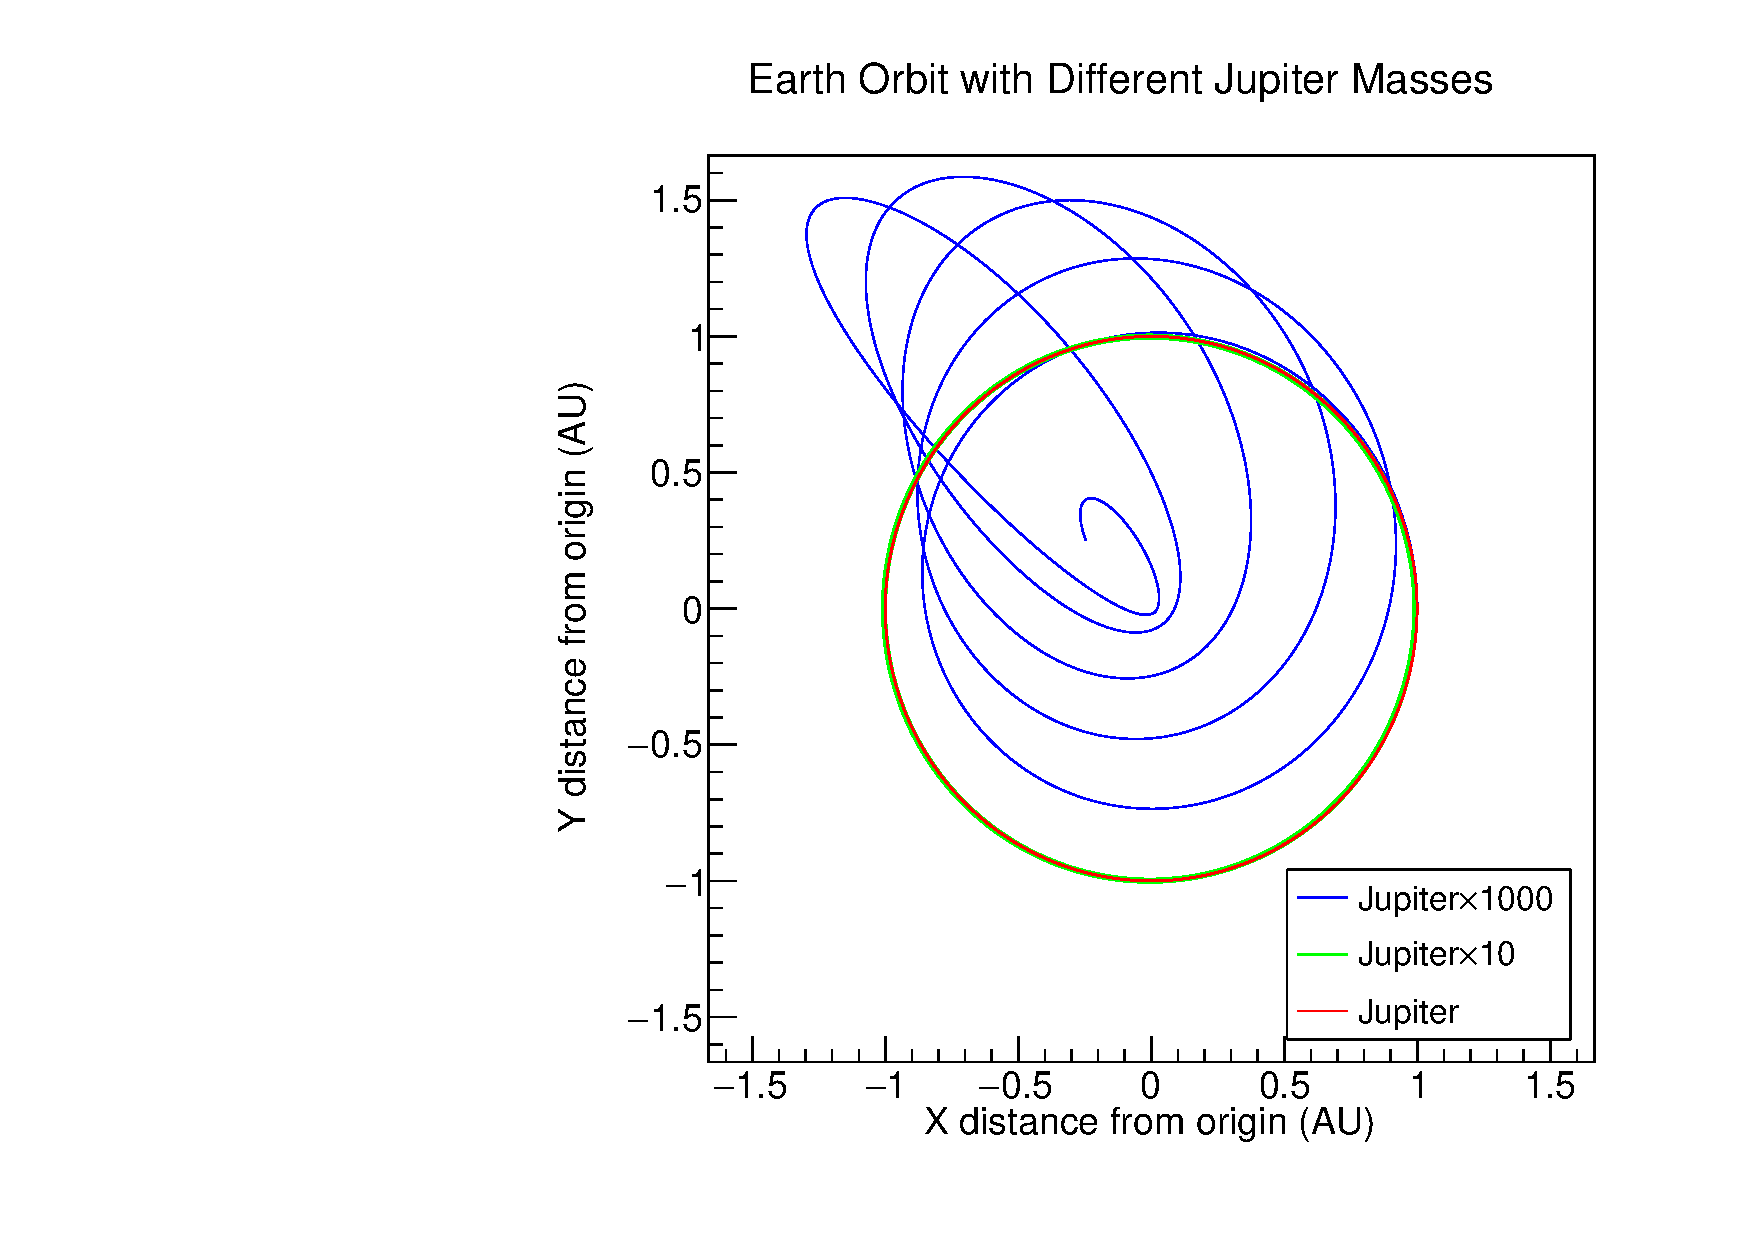
\includegraphics[width=0.5\textwidth]{ESJFVerlet_Earths.pdf}
  \caption{Plot of the position of earth in three body system with stationary sun and different Jupiter masses. Used a time length of 13 years with 13000 time steps with the Verlet algorithm.}
  \label{fig:ESJFVerlet_Earths}
 \end{SCfigure}

In figures \ref{fig:ESJFRK4_Earths} and \ref{fig:ESJFVerlet_Earths}, this method was applied in a system similar to that in section \ref{ssec:esf}, except that the planet, Jupiter, was added. To see the effect of the additional force on Earth, I have included Earth's orbit in cases where Jupiter's mass is different orders of magnitude greater than it is in reality. As can be seen, when Jupiter has a mass on the same order as the Sun, it destabilizes Earth's orbit using both the RK4 and Verlet algorithms, causing it to spiral in towards the Sun. 
\subsection{Three Body System: Dynamic Sun}\label{ssec:3bsds}

Here, the same procedure was carried out as in section \ref{ssec:3bsss} with the regular Jupiter mass, with the exception of allowing the Sun to move. To keep the system stable, the Sun was taken to have a position such that the position of Earth and Jupiter were measured from the center-of-mass of the solar system ( instead of distance from the Sun ), and a velocity such that the momentum of the entire system was zero. 

 \begin{SCfigure}
 \centering
   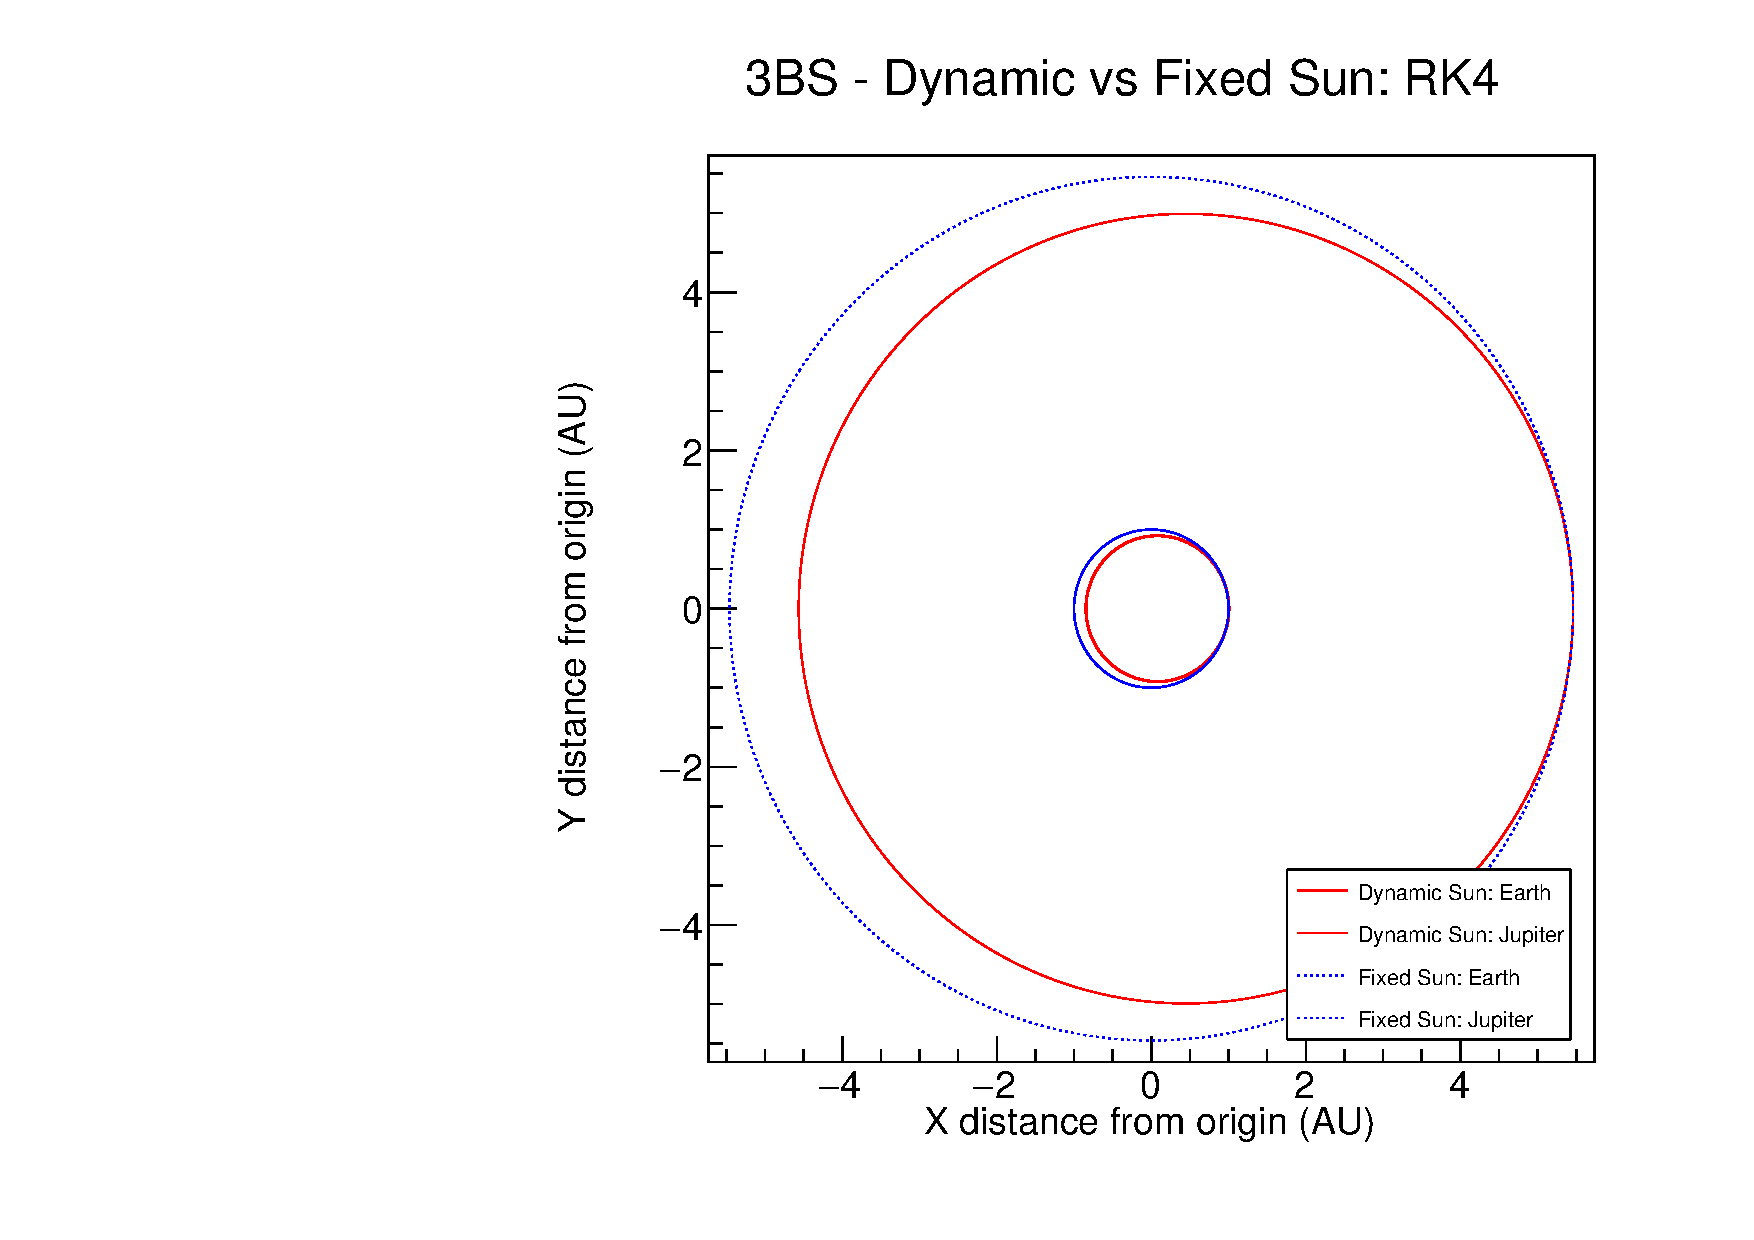
\includegraphics[width=0.5\textwidth]{ESJD_vs_ESJF_RK4.pdf}
  \caption{Plot comparing 3 body systems ( Earth, Jupiter, and the Sun ) with a stationary sun vs a system revolving around a common center of mass. Note the mass of the sun in the dynamic case was increased by 10\% to increase the visual effect. Time: 13 years, Time Steps:13000, Algorithm: RK4}
  \label{fig:ESJD_vs_ESJF_RK4}
 \end{SCfigure}

 
  \begin{SCfigure}
 \centering
   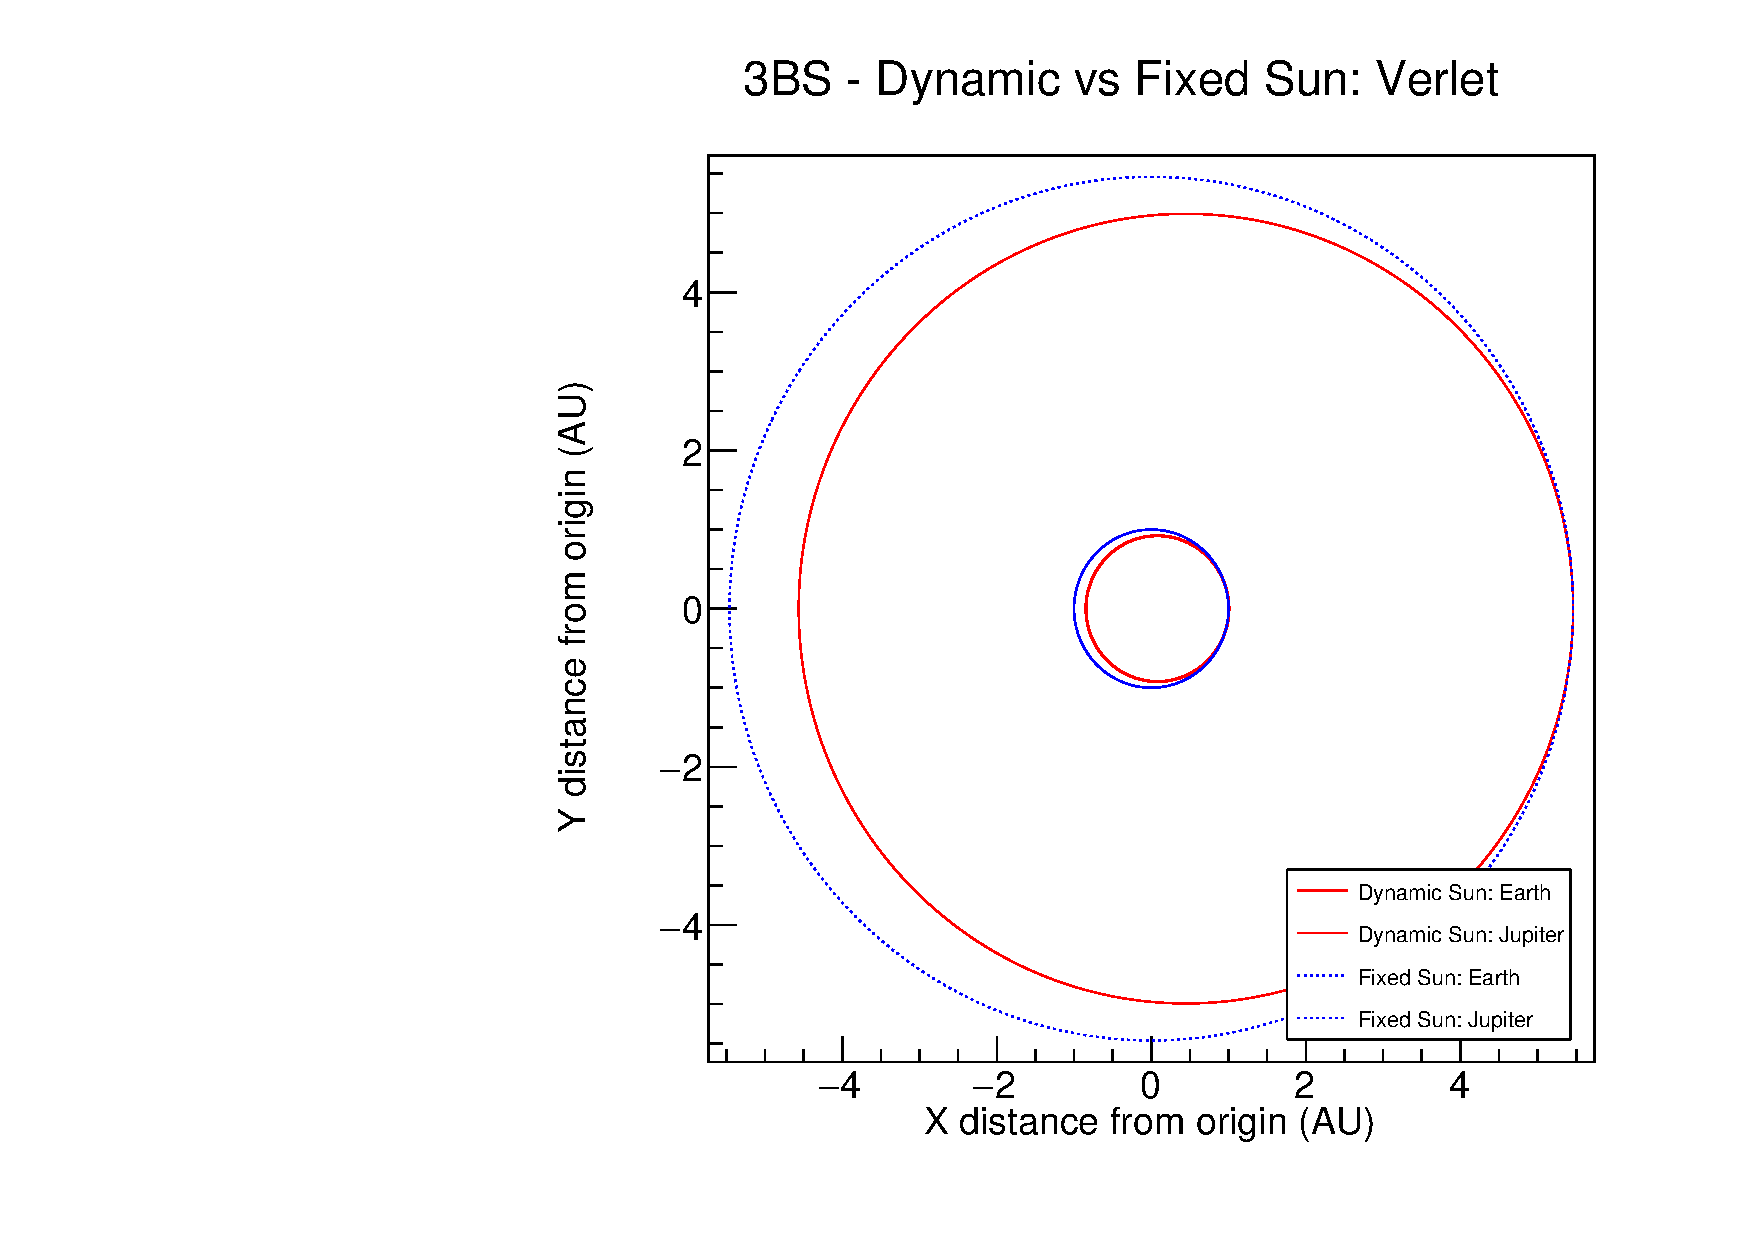
\includegraphics[width=0.5\textwidth]{ESJD_vs_ESJF_Verlet.pdf}
  \caption{Plot comparing 3 body systems ( Earth, Jupiter, and the Sun ) with a stationary sun vs a system revolving around a common center of mass. Note the mass of the sun in the dynamic case was increased by 10\% to increase the visual effect. Time: 13 years, Time Steps:13000, Algorithm: Verlet}
  \label{fig:ESJD_vs_ESJF_Verlet}
 \end{SCfigure}

 The results for the RK4 and Verlet algorithms turned out basically identical, as seen in plots \ref{fig:ESJD_vs_ESJF_RK4} and \ref{fig:ESJD_vs_ESJF_Verlet}. For effect, I increased the mass of the Sun in the dynamic case by 10\% to show that the orbits in the dynamic sun case are no longer centered at the origin, as would be expected with a stationary sun.
 
\subsection{All Major Solar System Bodies}

With a method to handle the many body case, it was not difficult to extend the three-body case to the set of all major bodies in the solar system.
  \begin{SCfigure}
 \centering
   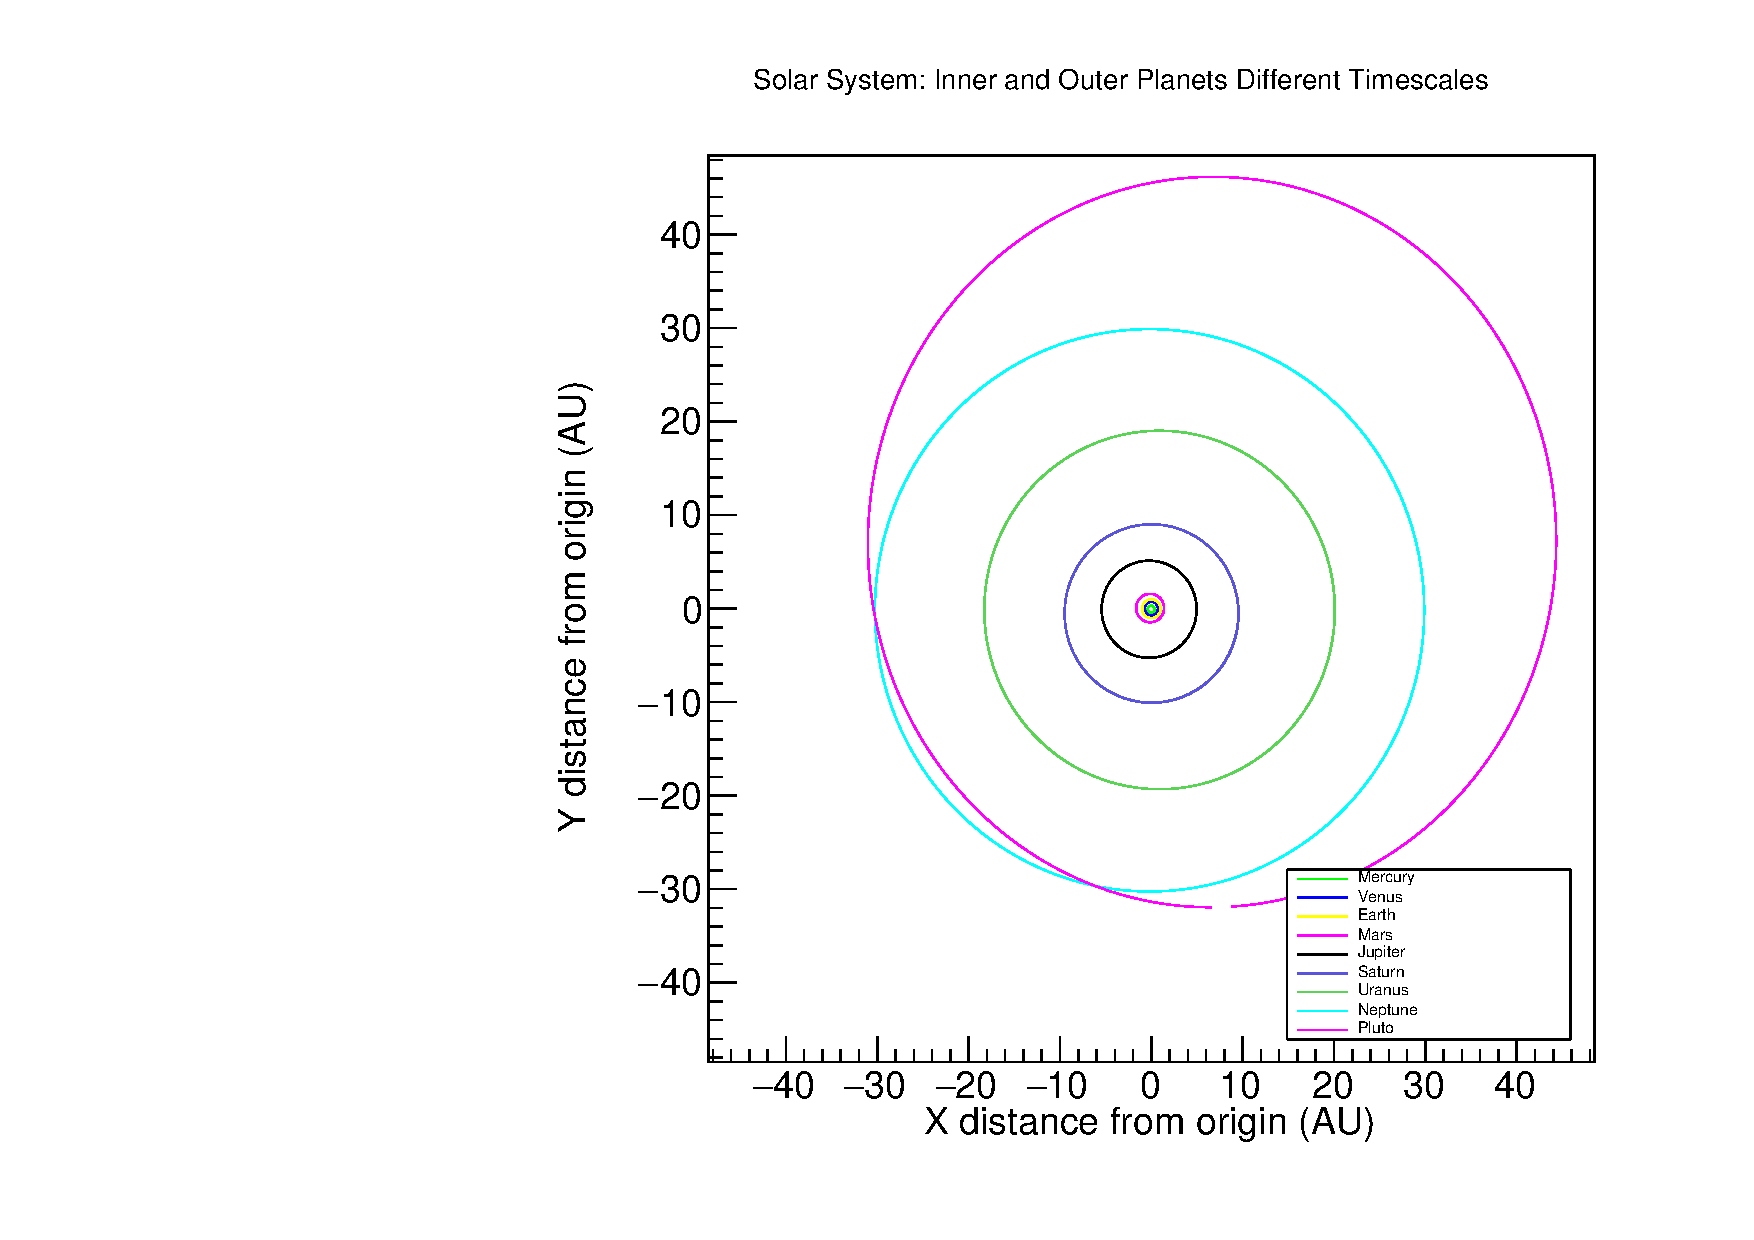
\includegraphics[width=0.5\textwidth]{all_bodies_inner_outer_sep_RK4.pdf}
  \caption{Plot of all major bodies with inner and outer planets calculated separately. Inner Planets - Time: 5 years, Time Steps: 5000, Algorithm: RK4. Outer Planets - Time: 250 years, Time Steps: 25000, Algorithm: RK4}
  \label{fig:all_bodies_inner_outer_sep_RK4}
 \end{SCfigure}

 \begin{SCfigure}
 \centering
   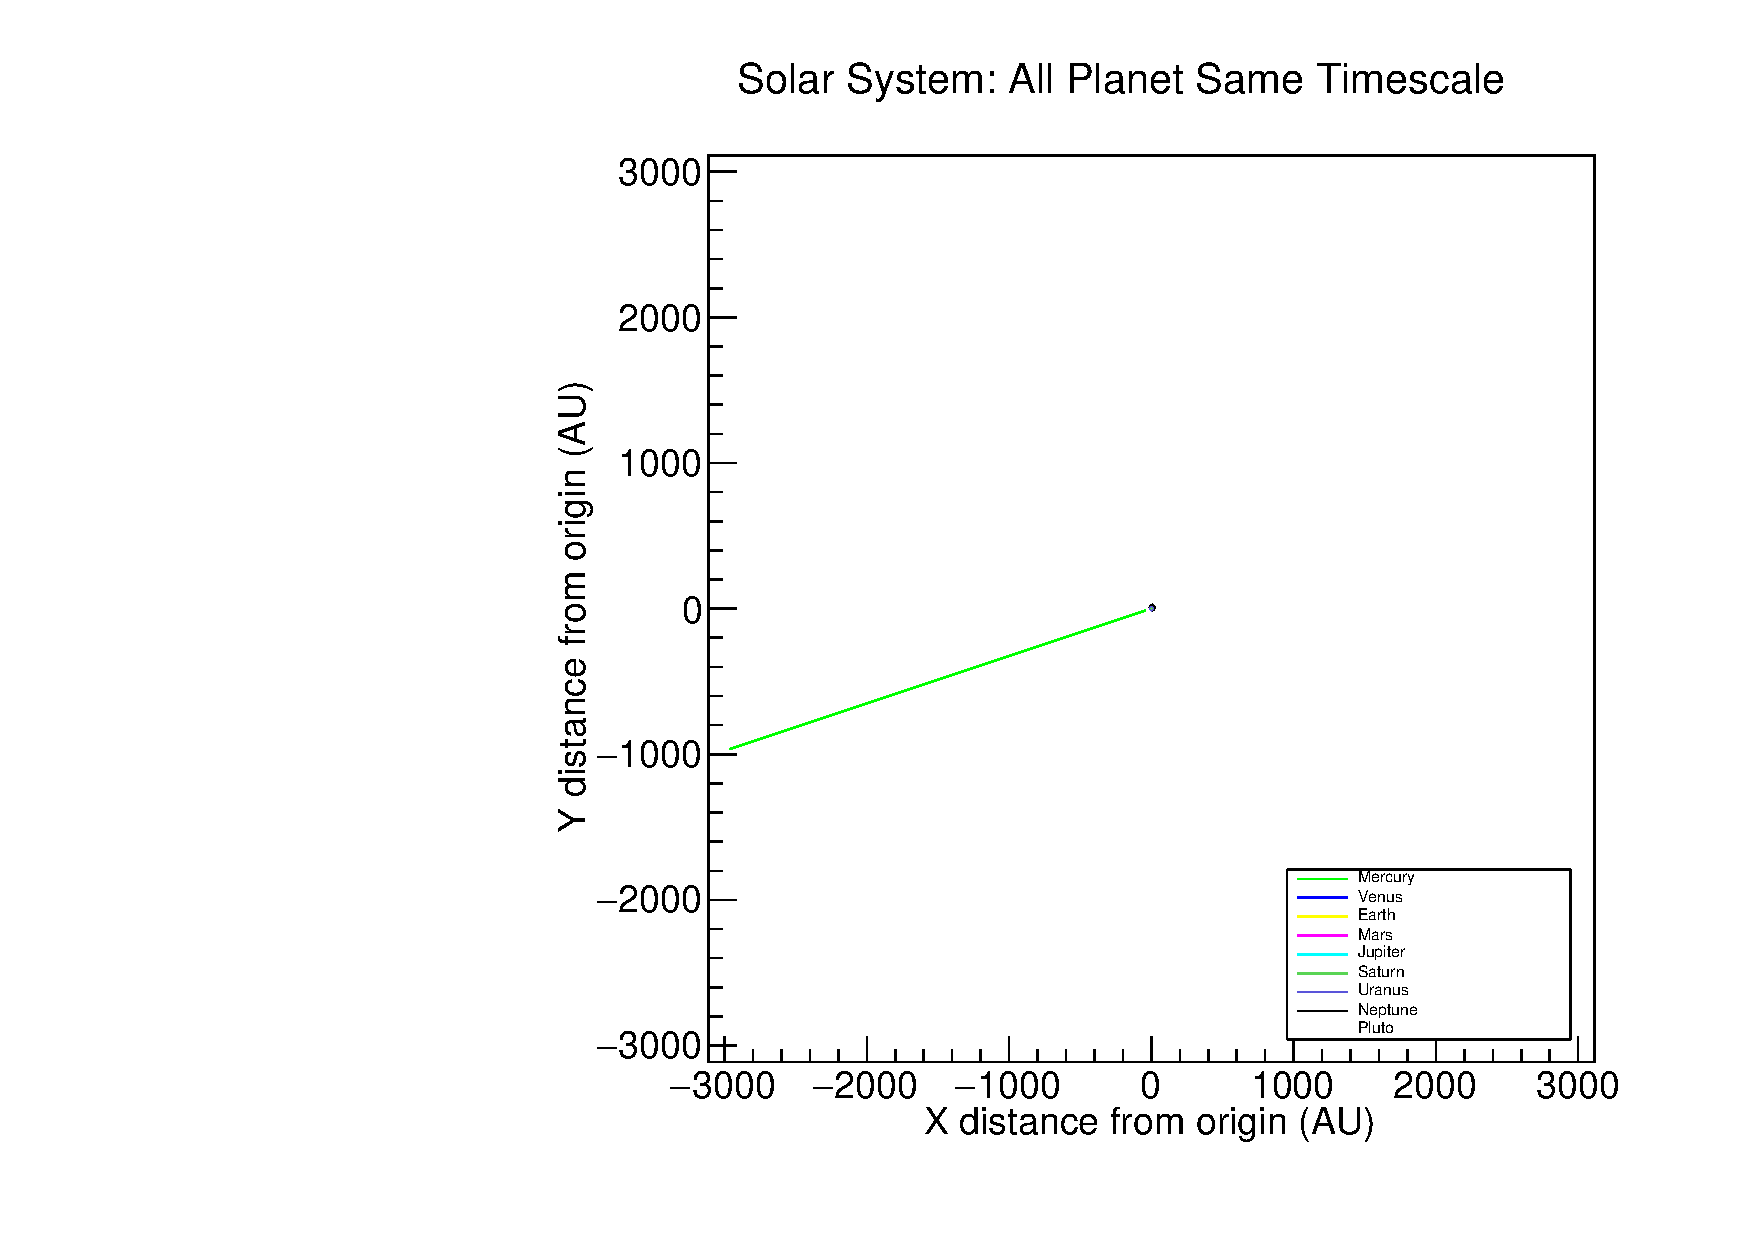
\includegraphics[width=0.5\textwidth]{all_bodies_same_time_RK4.pdf}
  \caption{Plot of all major bodies calculated at the same time. Note that Mercury leaves the solar system. Time: 250 years, Time Steps: 25000, Algorithm: RK4}
  \label{fig:all_bodies_same_time_RK4}
 \end{SCfigure}
 One difficulty arises when calculating the orbits of all major bodies with the fact that the distances and time scales of the solar system span 3-4 orders of magnitude. Hence, what might be a relatively short time step for Pluto is also the time of several periods of Mercury's orbit. This can be seen in figure \ref{fig:all_bodies_same_time_RK4}, where Mercury leaves the solar system due to this problem. To remedy this, I calculated the orbits of the inner and outer solar system separately to get figure \ref{fig:all_bodies_inner_outer_sep_RK4}. Also, note that using the Verlet algorithm in figure \ref{fig:all_bodies_same_time_Verlet} doesn't cause Mercury to leave the solar system. Based on figures \ref{fig:ESVerlet_pe} and \ref{fig:ESVerlet_ke} This seems to be due to the fact that the Verlet algorithm causes the potential energy to blow up and the kinetic energy to go down with coarse time steps. This would cause Mercury to crash into the Sun, instead of leave the solar system.
 
\section{Conclusion}\label{sec:conclude}
Both algorithms give good approximations of orbits in single and many body cases given sufficient time steps. The RK4 method is more exact that the Verlet method at the expense of being more difficult to utilize and some extra floating point operations ( both algorithms only depend on the previous step, so they only increase in floating point operations linearly ). The many body case is limited by systems that move at many different timescales, since a relatively short time step for a body with a long period is a long time step for a body with a short period. The algorithms also fail to take into account effects due to general relativity. Both of these shortcomings can be seen in figure \ref{fig:all_bodies_same_time_RK4} with Mercury. 

The different time scales can be remedied by calculating the orbits of bodies on different time scales separately. This is the method used in figure \ref{fig:all_bodies_inner_outer_sep_RK4}. Additionally, discrepancies due to general relativity could be remedied by including a relativistic correction to the calculation of the force on relevant bodies.

\appendix
\addtocontents{toc}{\protect\contentsline{chapter}{Appendix:}{}}
\chapter{Earth-Sun Plots}\label{app:esplots}

\begin{figure}[H]
 \centering
   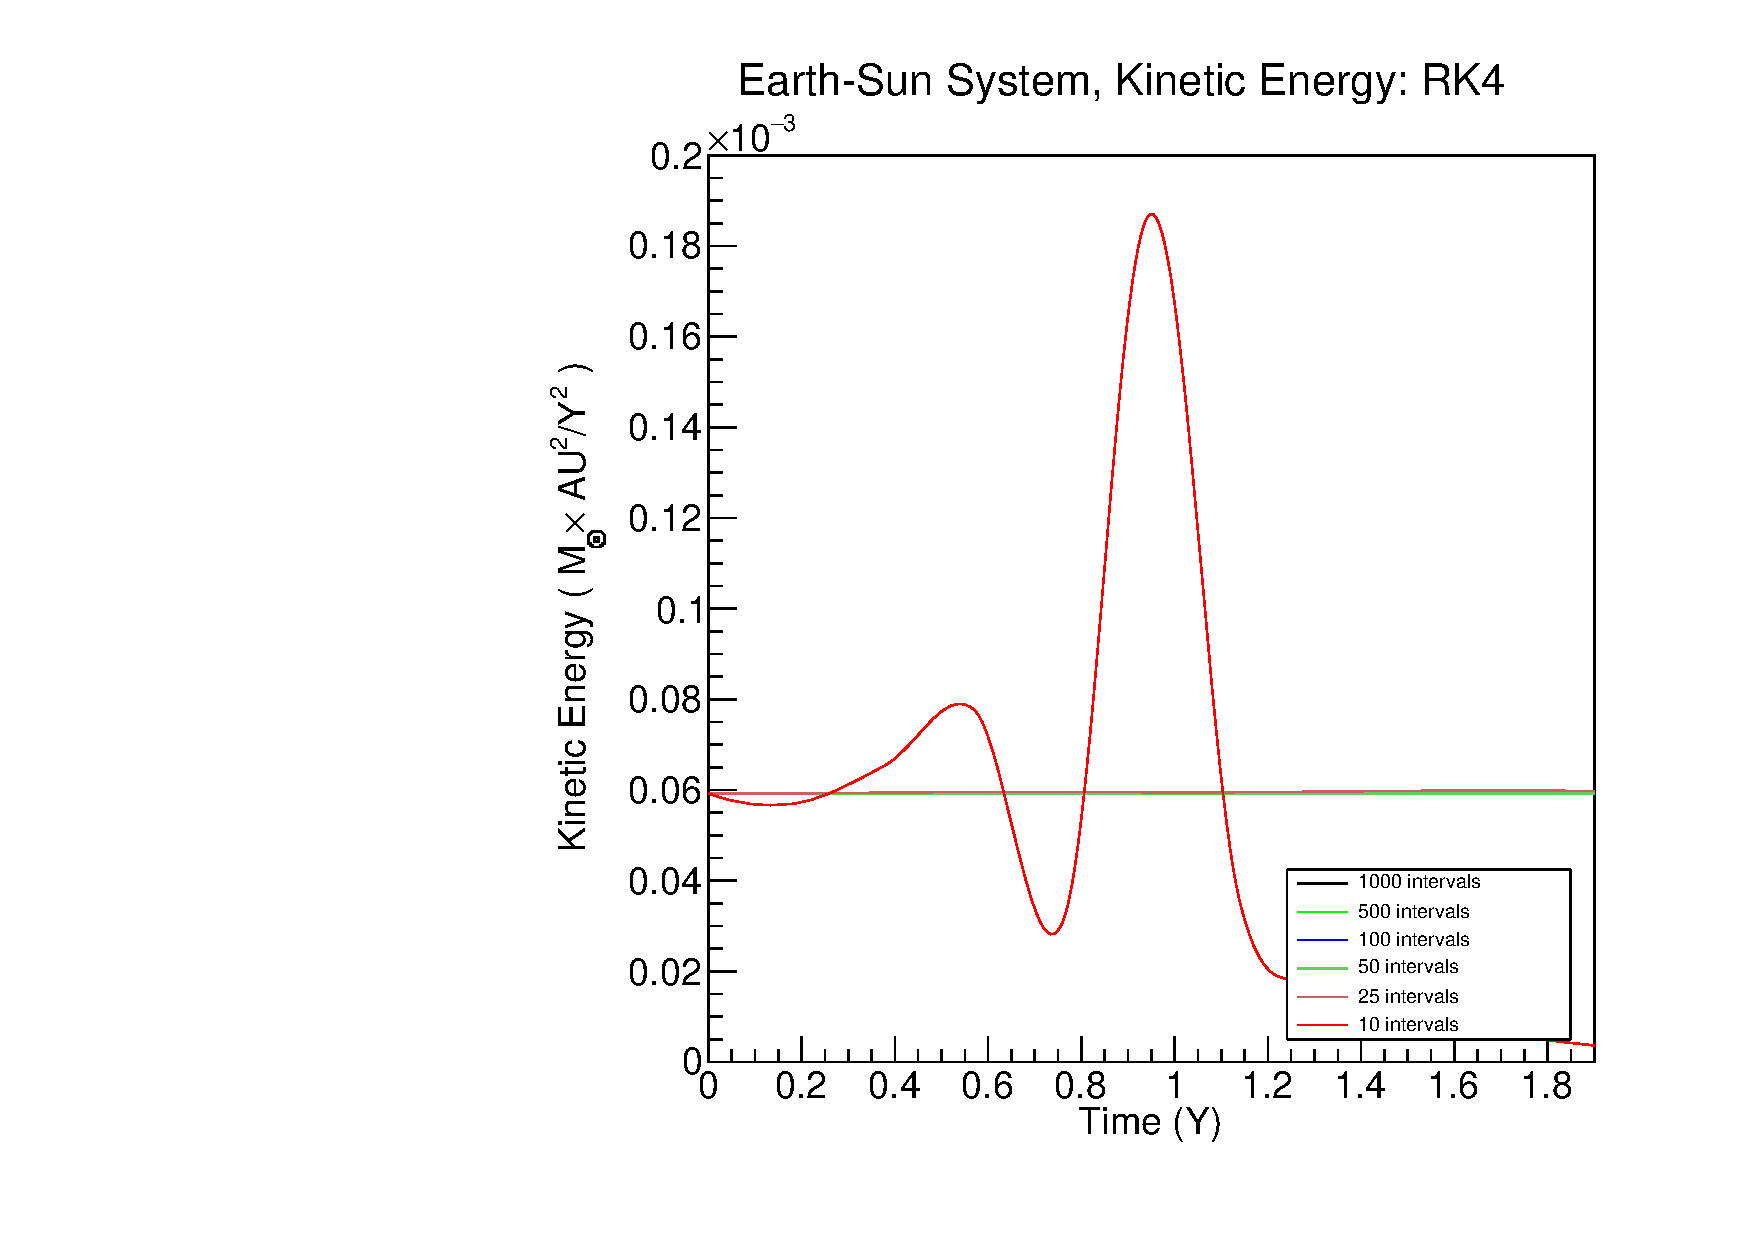
\includegraphics[width=0.5\textwidth]{ESRK4_ke.pdf}
  \caption{Plot of Earth-Sun system kinetic energy for different numbers of time steps over 1.9 years using the RK4 algorithm.}
  \label{fig:ESRK4_ke}
 \end{figure}
 
   \begin{figure}[H]
 \centering
   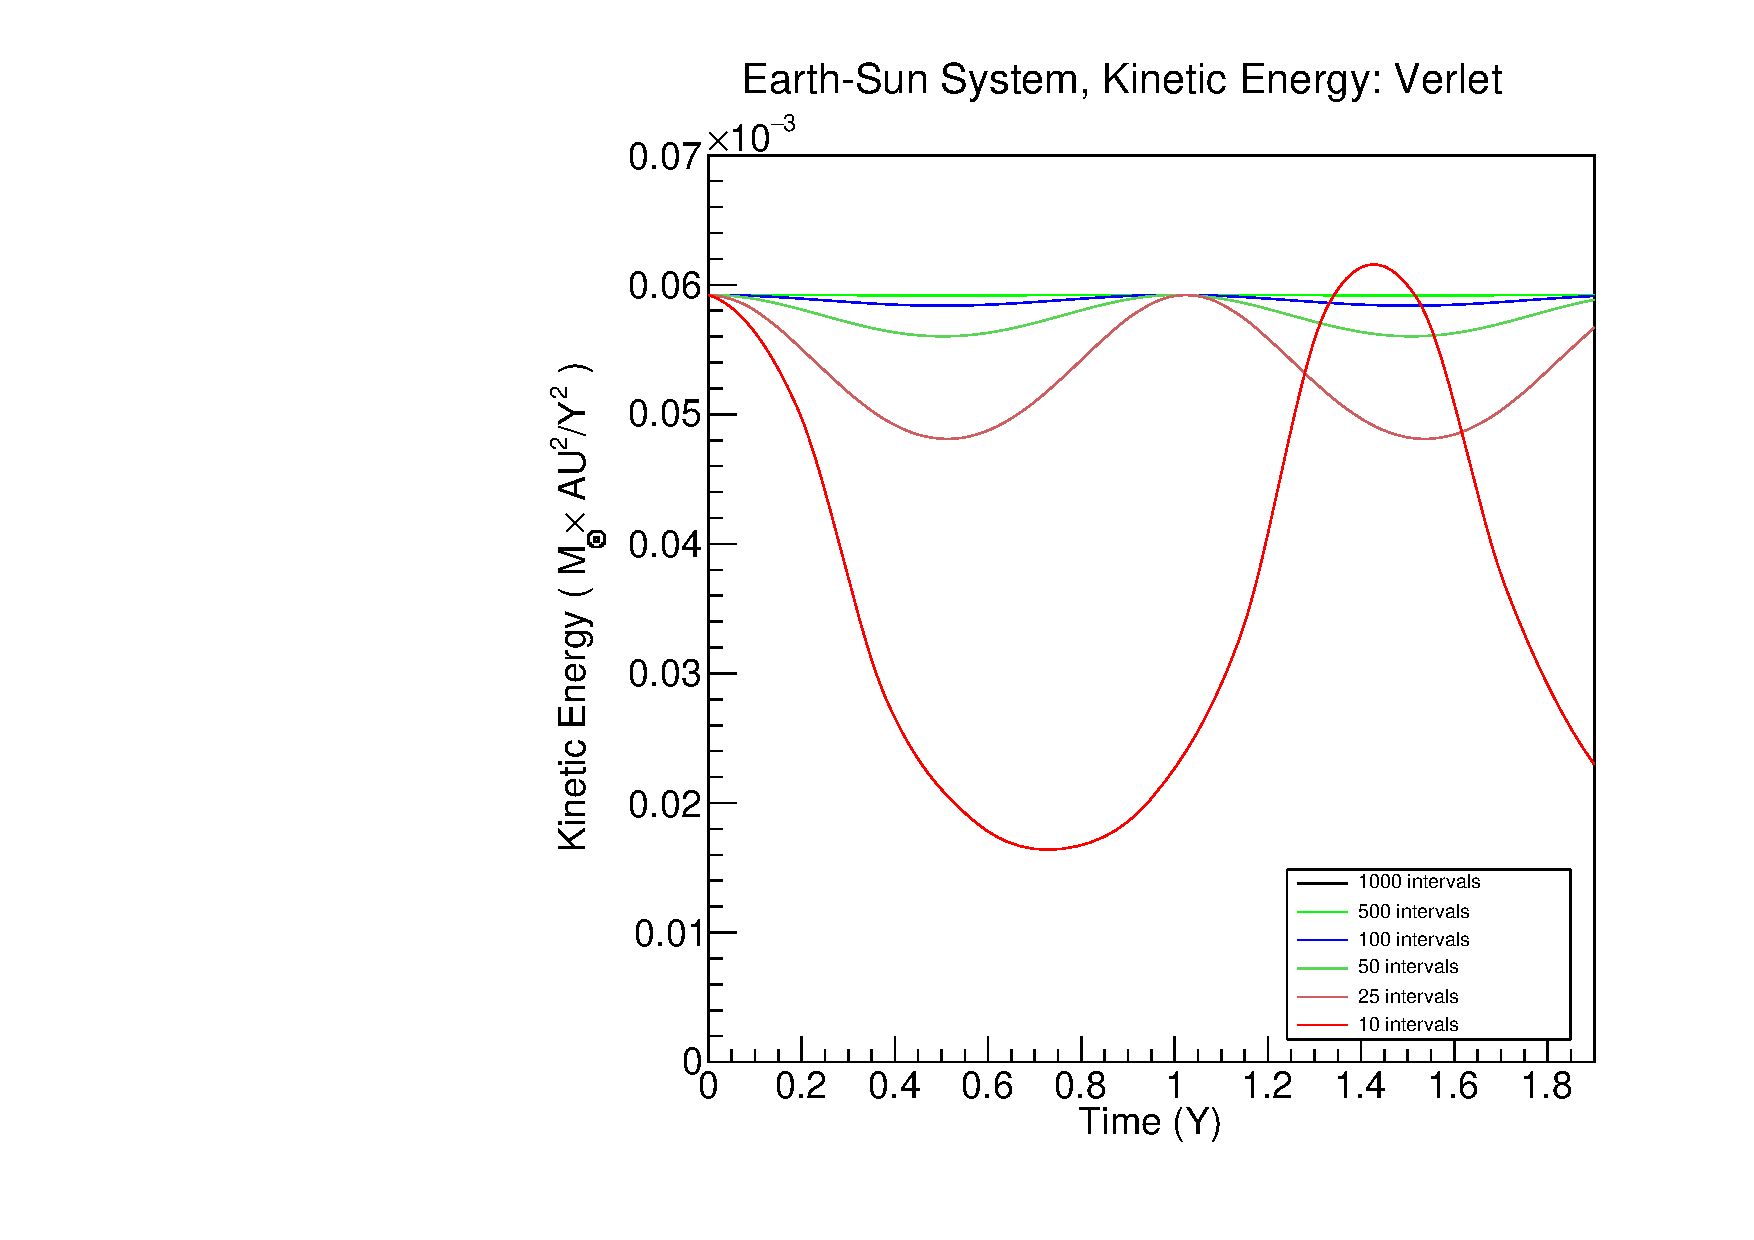
\includegraphics[width=0.5\textwidth]{ESVerlet_ke.pdf}
  \caption{Plot of Earth-Sun system kinetic energy for different numbers of time steps over 1.9 years using the Verlet algorithm.}
  \label{fig:ESVerlet_ke}
 \end{figure}


\begin{figure}[H]
 \centering
   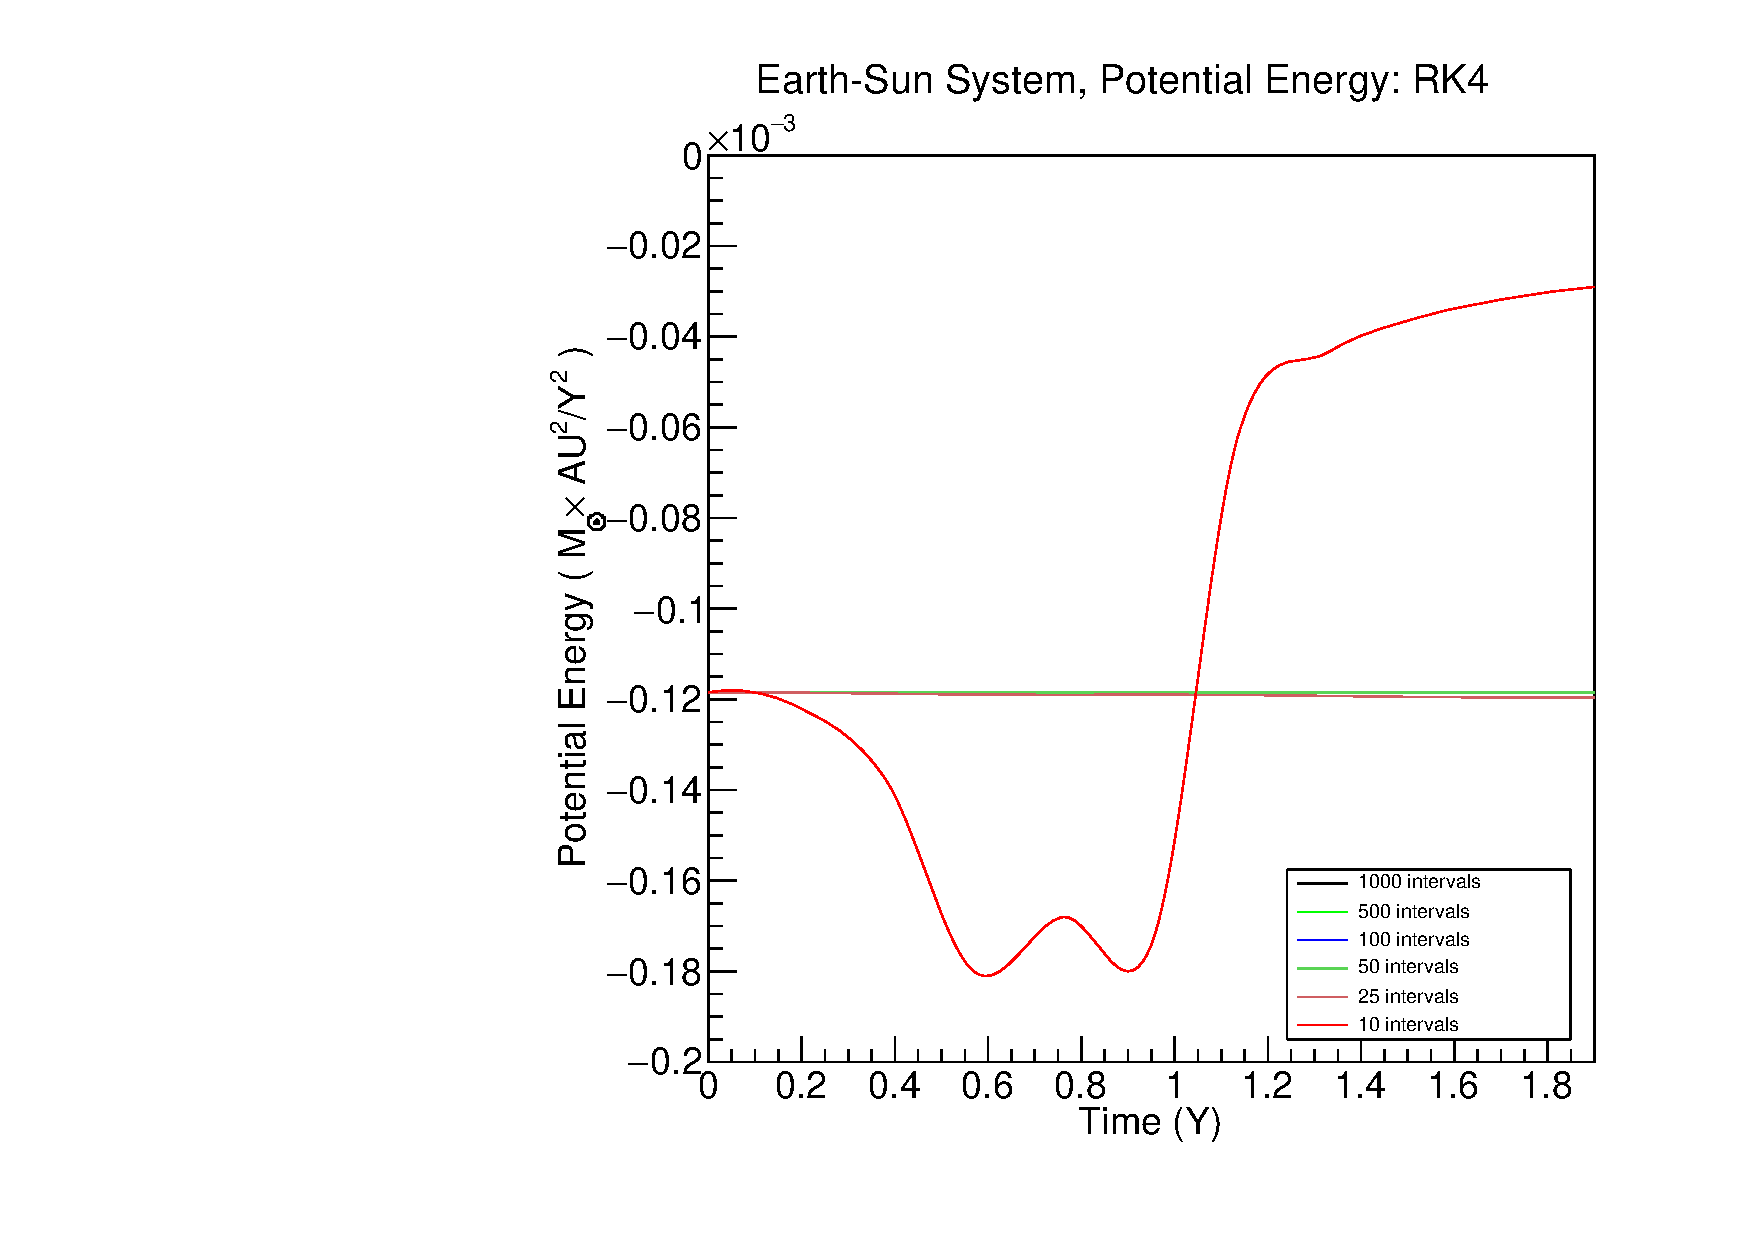
\includegraphics[width=0.5\textwidth]{ESRK4_pe.pdf}
  \caption{Plot of Earth-Sun system potential energy for different numbers of time steps over 1.9 years using the RK4 algorithm.}
  \label{fig:ESRK4_pe}
 \end{figure}

 \begin{figure}[H]
 \centering
   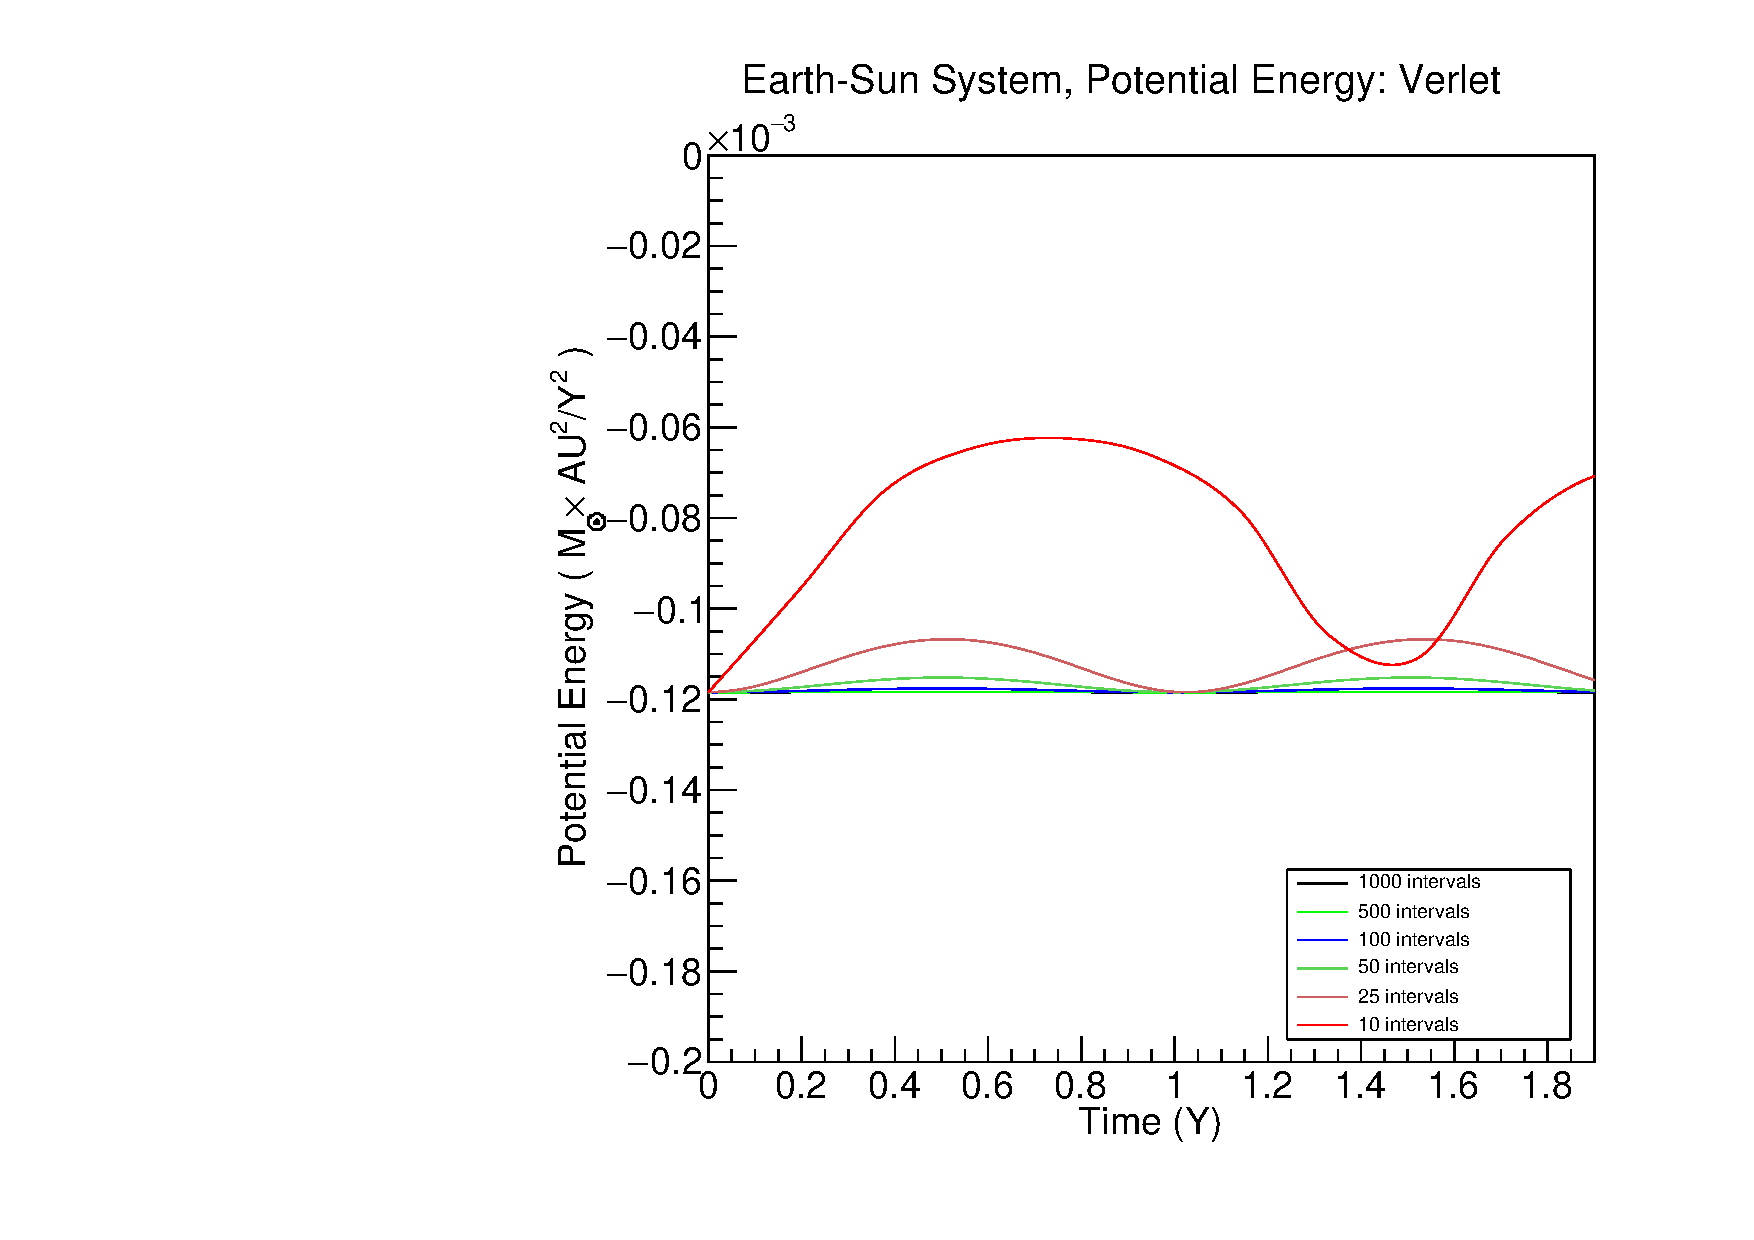
\includegraphics[width=0.5\textwidth]{ESVerlet_pe.pdf}
  \caption{Plot of Earth-Sun system potential energy for different numbers of time steps over 1.9 years using the Verlet algorithm.}
  \label{fig:ESVerlet_pe}
 \end{figure}

\begin{figure}[H]
 \centering
   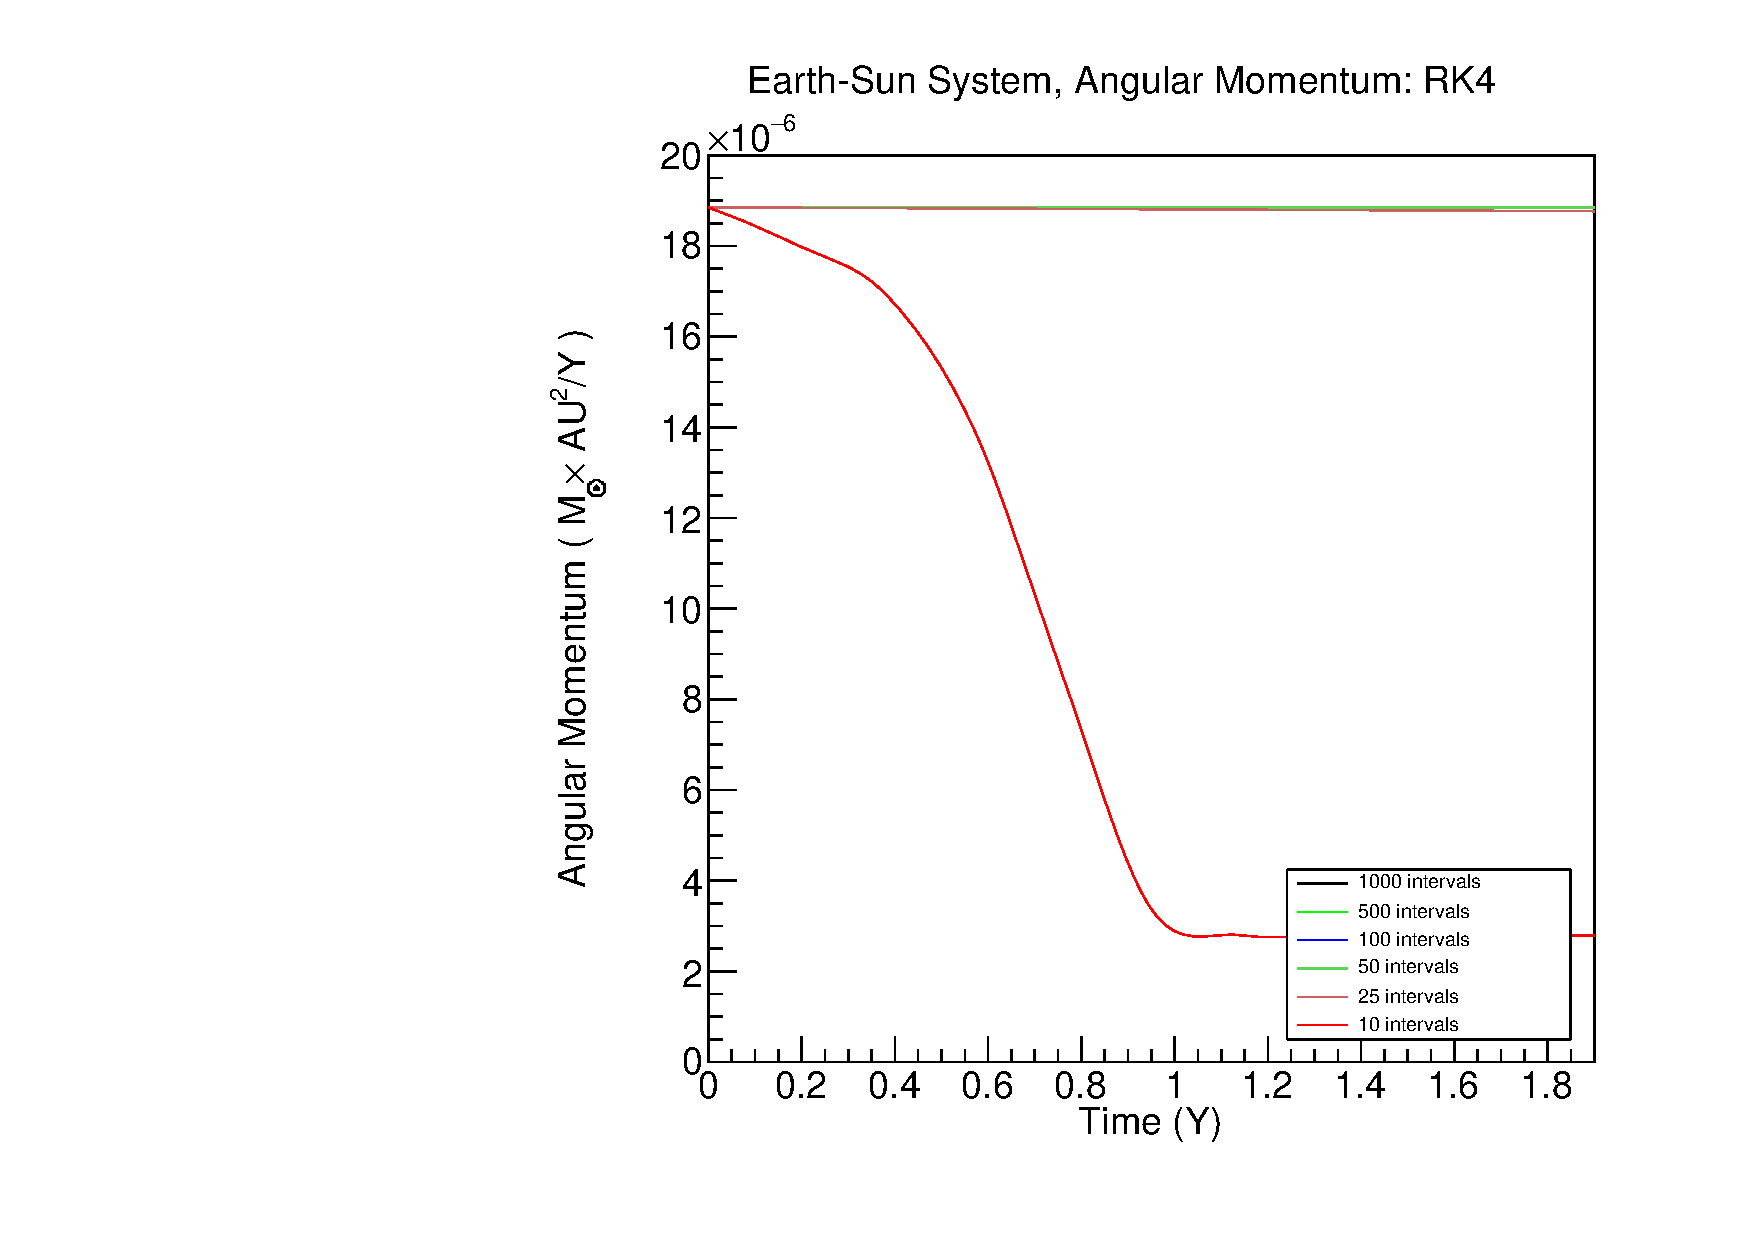
\includegraphics[width=0.5\textwidth]{ESRK4_l.pdf}
  \caption{Plot of Earth-Sun system angular momentum for different numbers of time steps over 1.9 years using the RK4 algorithm.}
  \label{fig:ESRK4_l}
 \end{figure}



\begin{figure}[H]
 \centering
   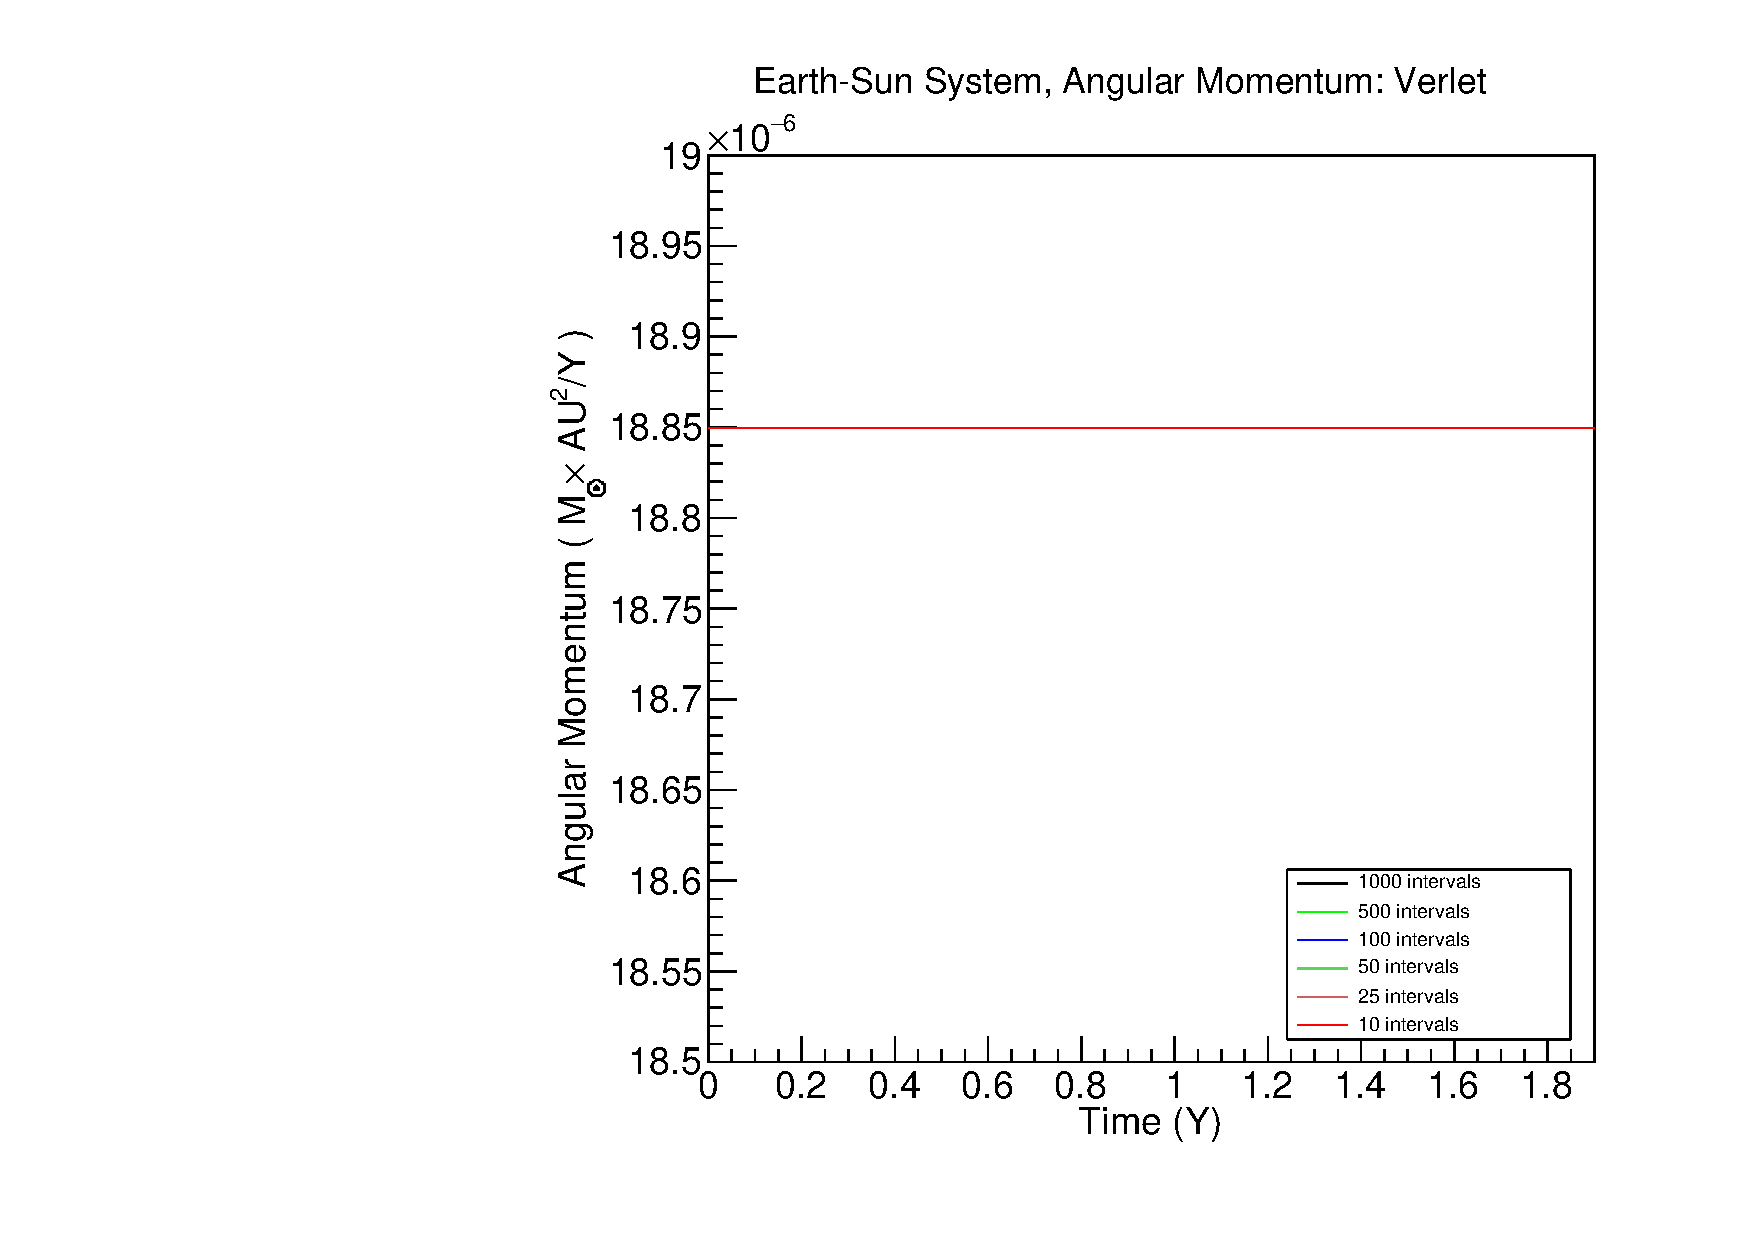
\includegraphics[width=0.5\textwidth]{ESVerlet_l.pdf}
  \caption{Plot of Earth-Sun system angular momentum for different numbers of time steps over 1.9 years using the Verlet algorithm.}
  \label{fig:ESVerlet_l}
 \end{figure}
 
 \chapter{Three Body System: Stationary Sun Plots}\label{app:3bsss}
 
 \begin{figure}[H]
 \centering
   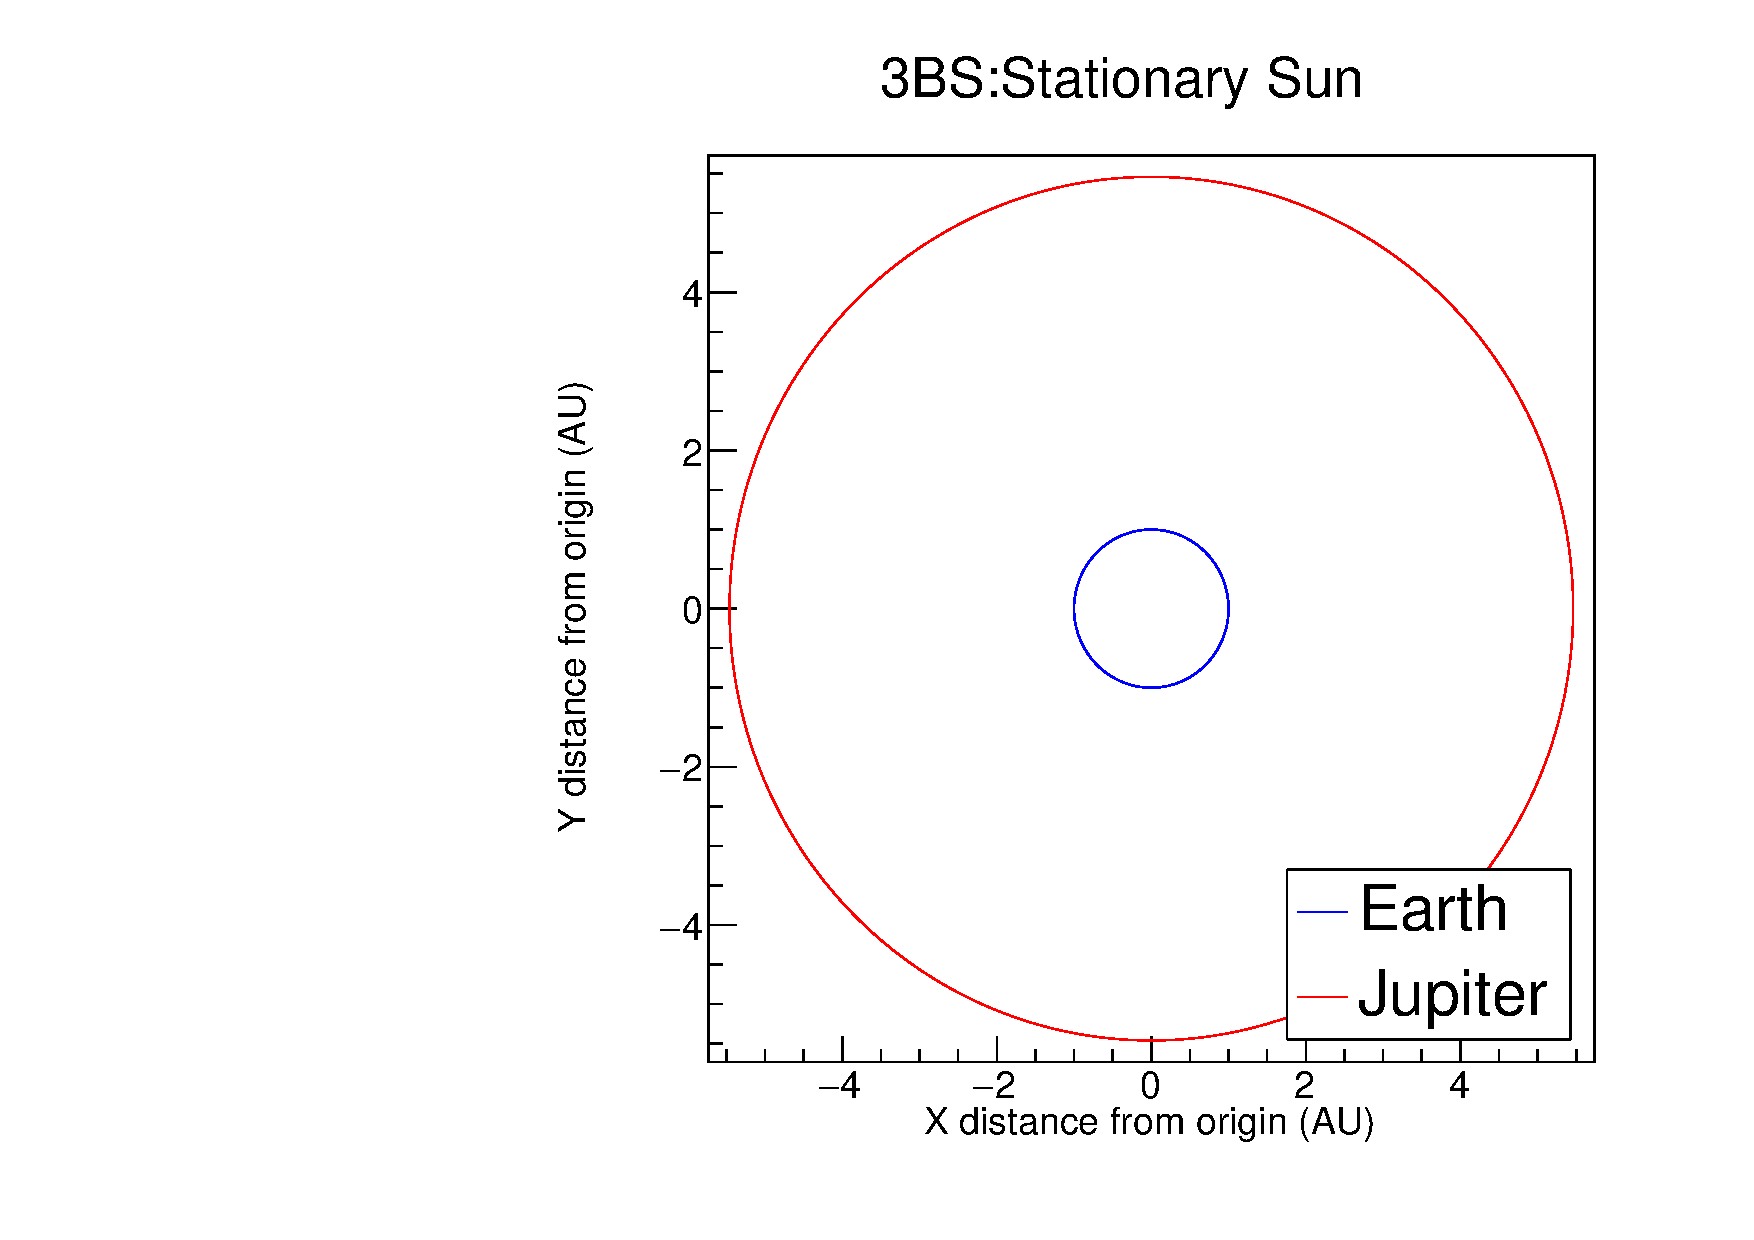
\includegraphics[width=0.5\textwidth]{ESJFRK4_reg.pdf}
  \caption{Plot of 3 body system with Earth, Jupiter, and a stationary sun using regular Jupiter mass. Time interval: 13 years, Time steps: 13000, Algorithm: RK4.}
  \label{fig:ESJFRK4_reg}
 \end{figure}
 
  \begin{figure}[H]
 \centering
   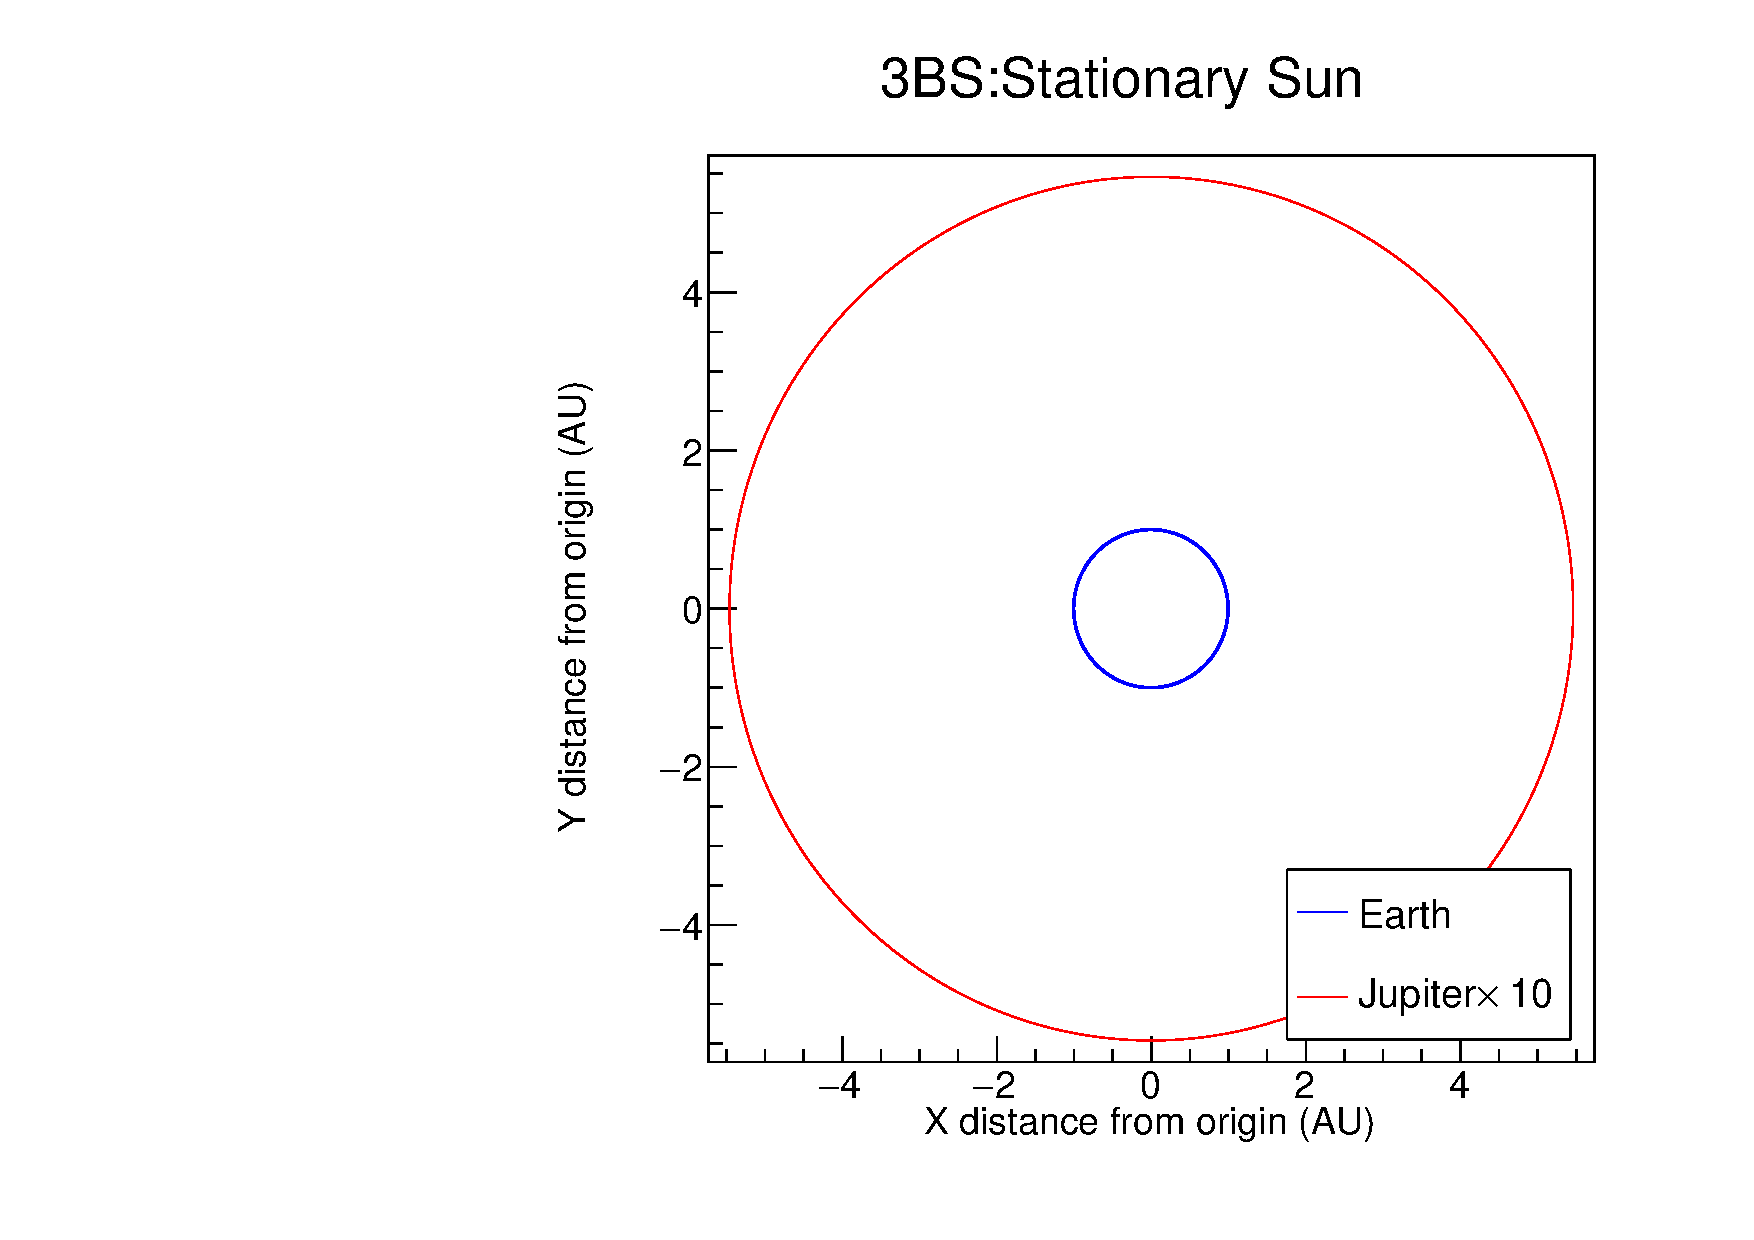
\includegraphics[width=0.5\textwidth]{ESJFRK4_x10.pdf}
  \caption{Plot of 3 body system with Earth, Jupiter, and a stationary sun using $\times 10$ Jupiter mass. Time interval: 13 years, Time steps: 13000, Algorithm: RK4.}
  \label{fig:ESJFRK4_x10}
 \end{figure}
 
  \begin{figure}[H]
 \centering
   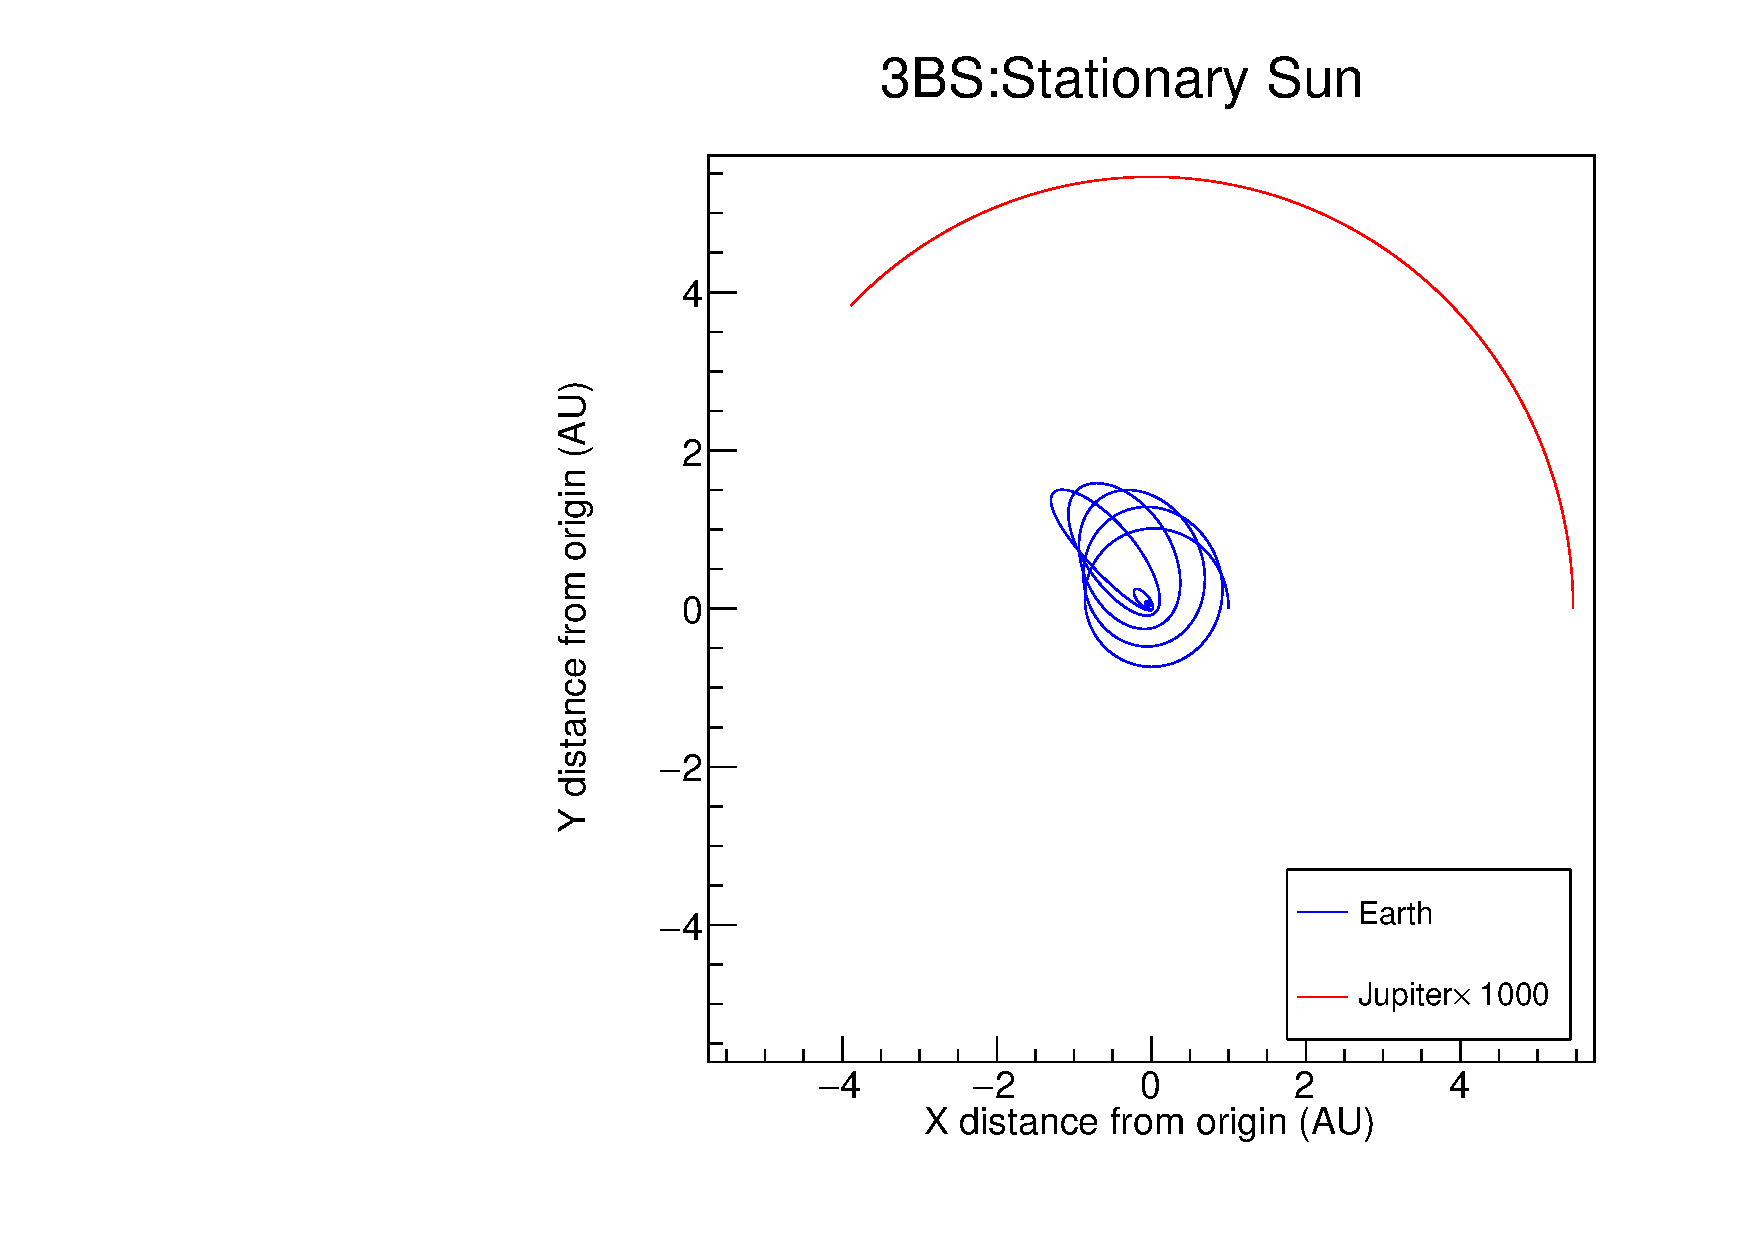
\includegraphics[width=0.5\textwidth]{ESJFRK4_x1000.pdf}
  \caption{Plot of 3 body system with Earth, Jupiter, and a stationary sun using $\times 1000$ Jupiter mass. Used a shorter timespan because this heavy Jupiter causes Earth to ``hit the sun'', then go barreling out many AU so the orbital structure is no longer visible. Time interval: 4.8 years, Time steps: 13000, Algorithm: RK4.}
  \label{fig:ESJFRK4_x1000}
 \end{figure}
 
 \begin{figure}[H]
 \centering
   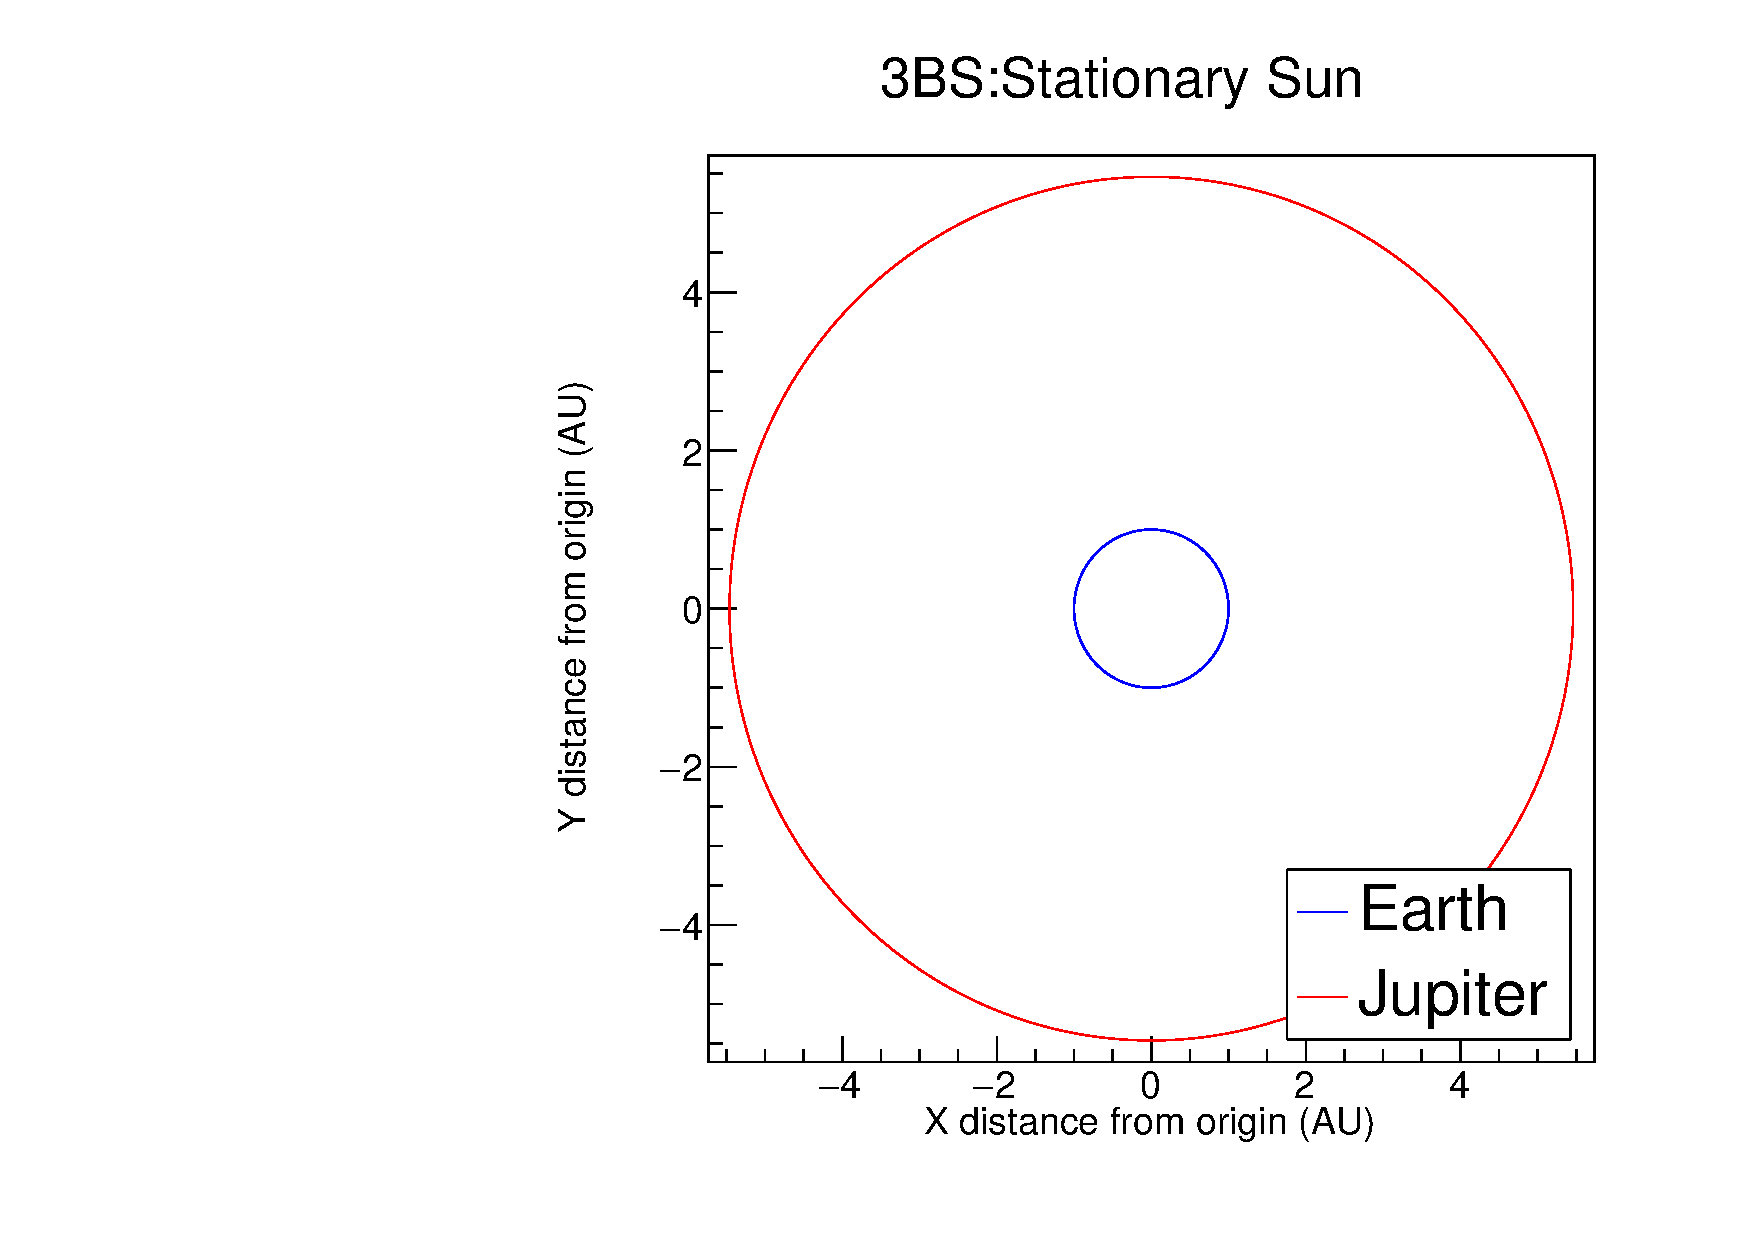
\includegraphics[width=0.5\textwidth]{ESJFVerlet_reg.pdf}
  \caption{Plot of 3 body system with Earth, Jupiter, and a stationary sun using regular Jupiter mass. Time interval: 13 years, Time steps: 13000, Algorithm: Verlet.}
  \label{fig:ESJFVerlet_reg}
 \end{figure}
 
  \begin{figure}[H]
 \centering
   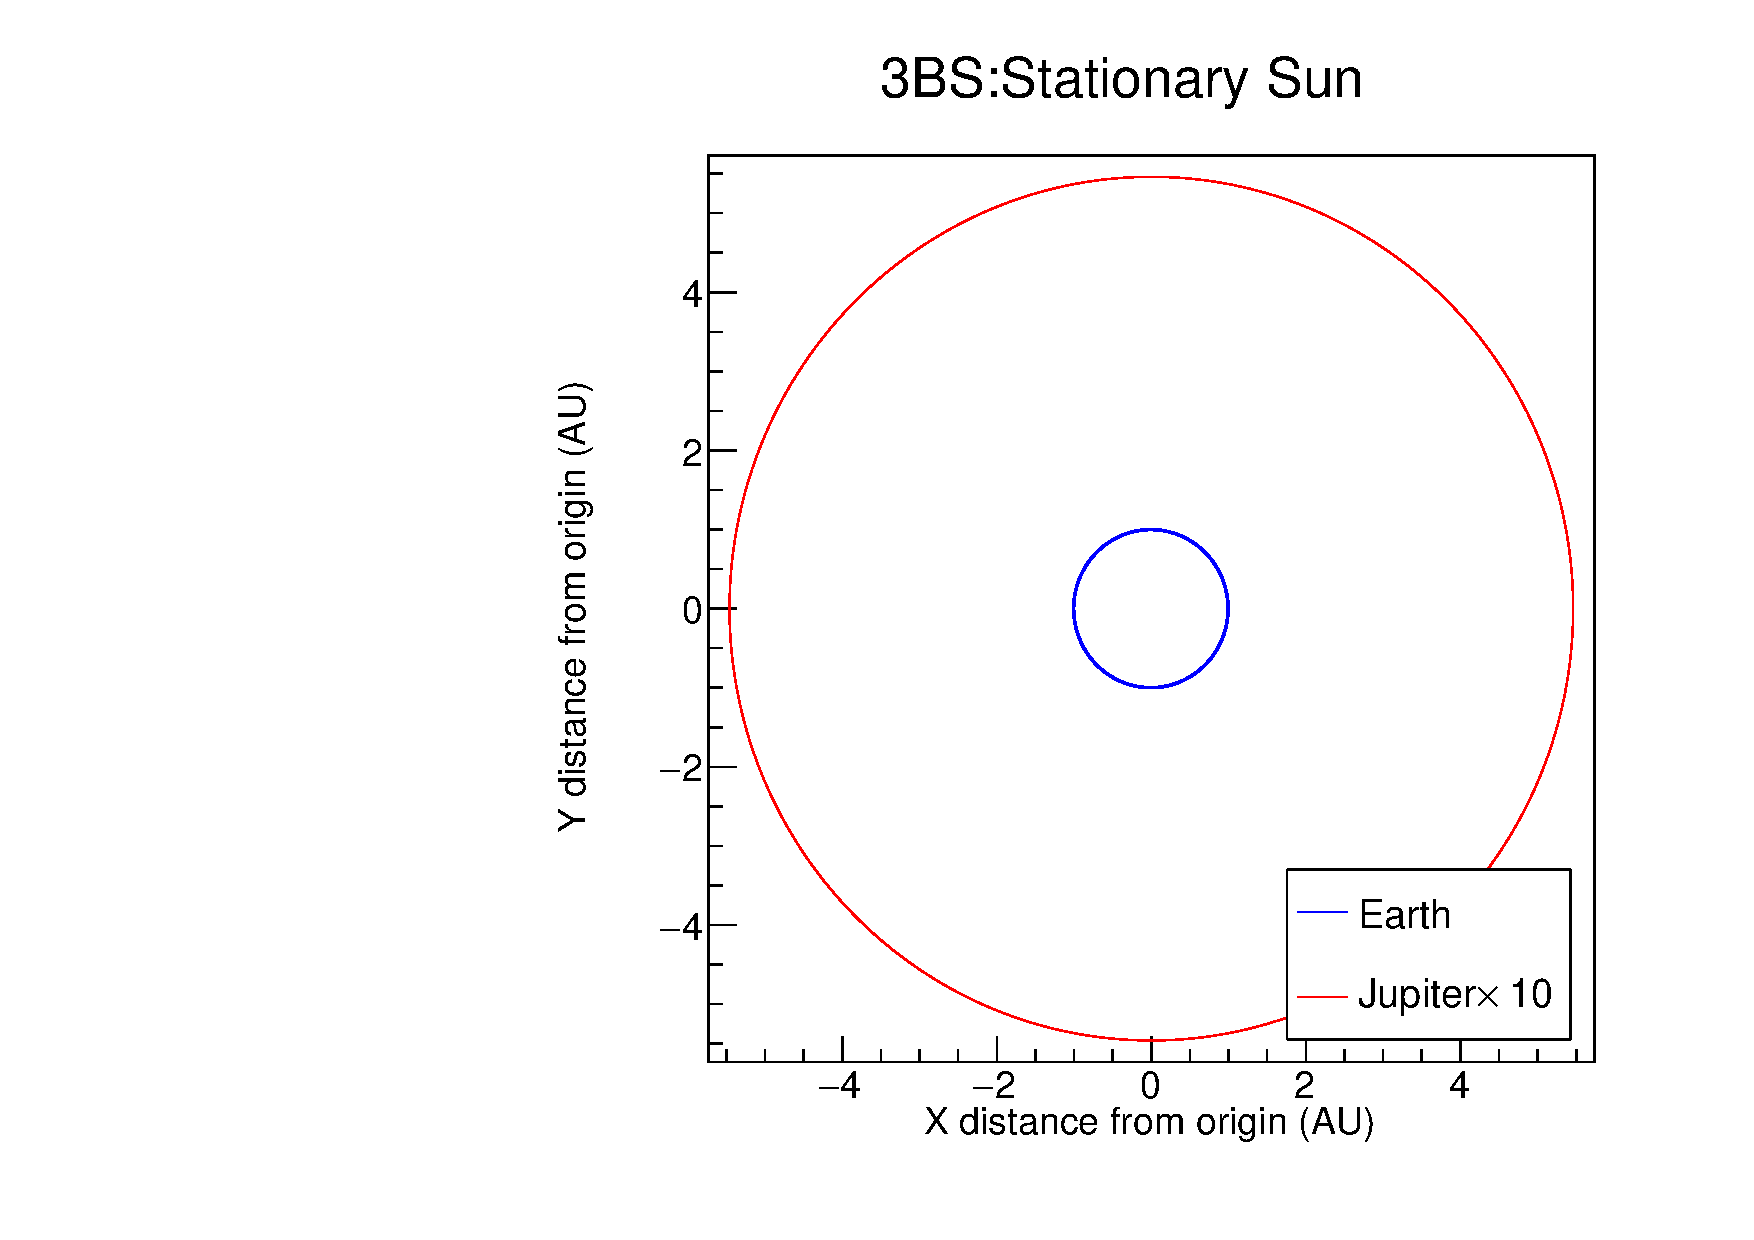
\includegraphics[width=0.5\textwidth]{ESJFVerlet_x10.pdf}
  \caption{Plot of 3 body system with Earth, Jupiter, and a stationary sun using $\times 10$ Jupiter mass. Time interval: 13 years, Time steps: 13000, Algorithm: Verlet.}
  \label{fig:ESJFVerlet_x10}
 \end{figure}
 
  \begin{figure}[H]
 \centering
   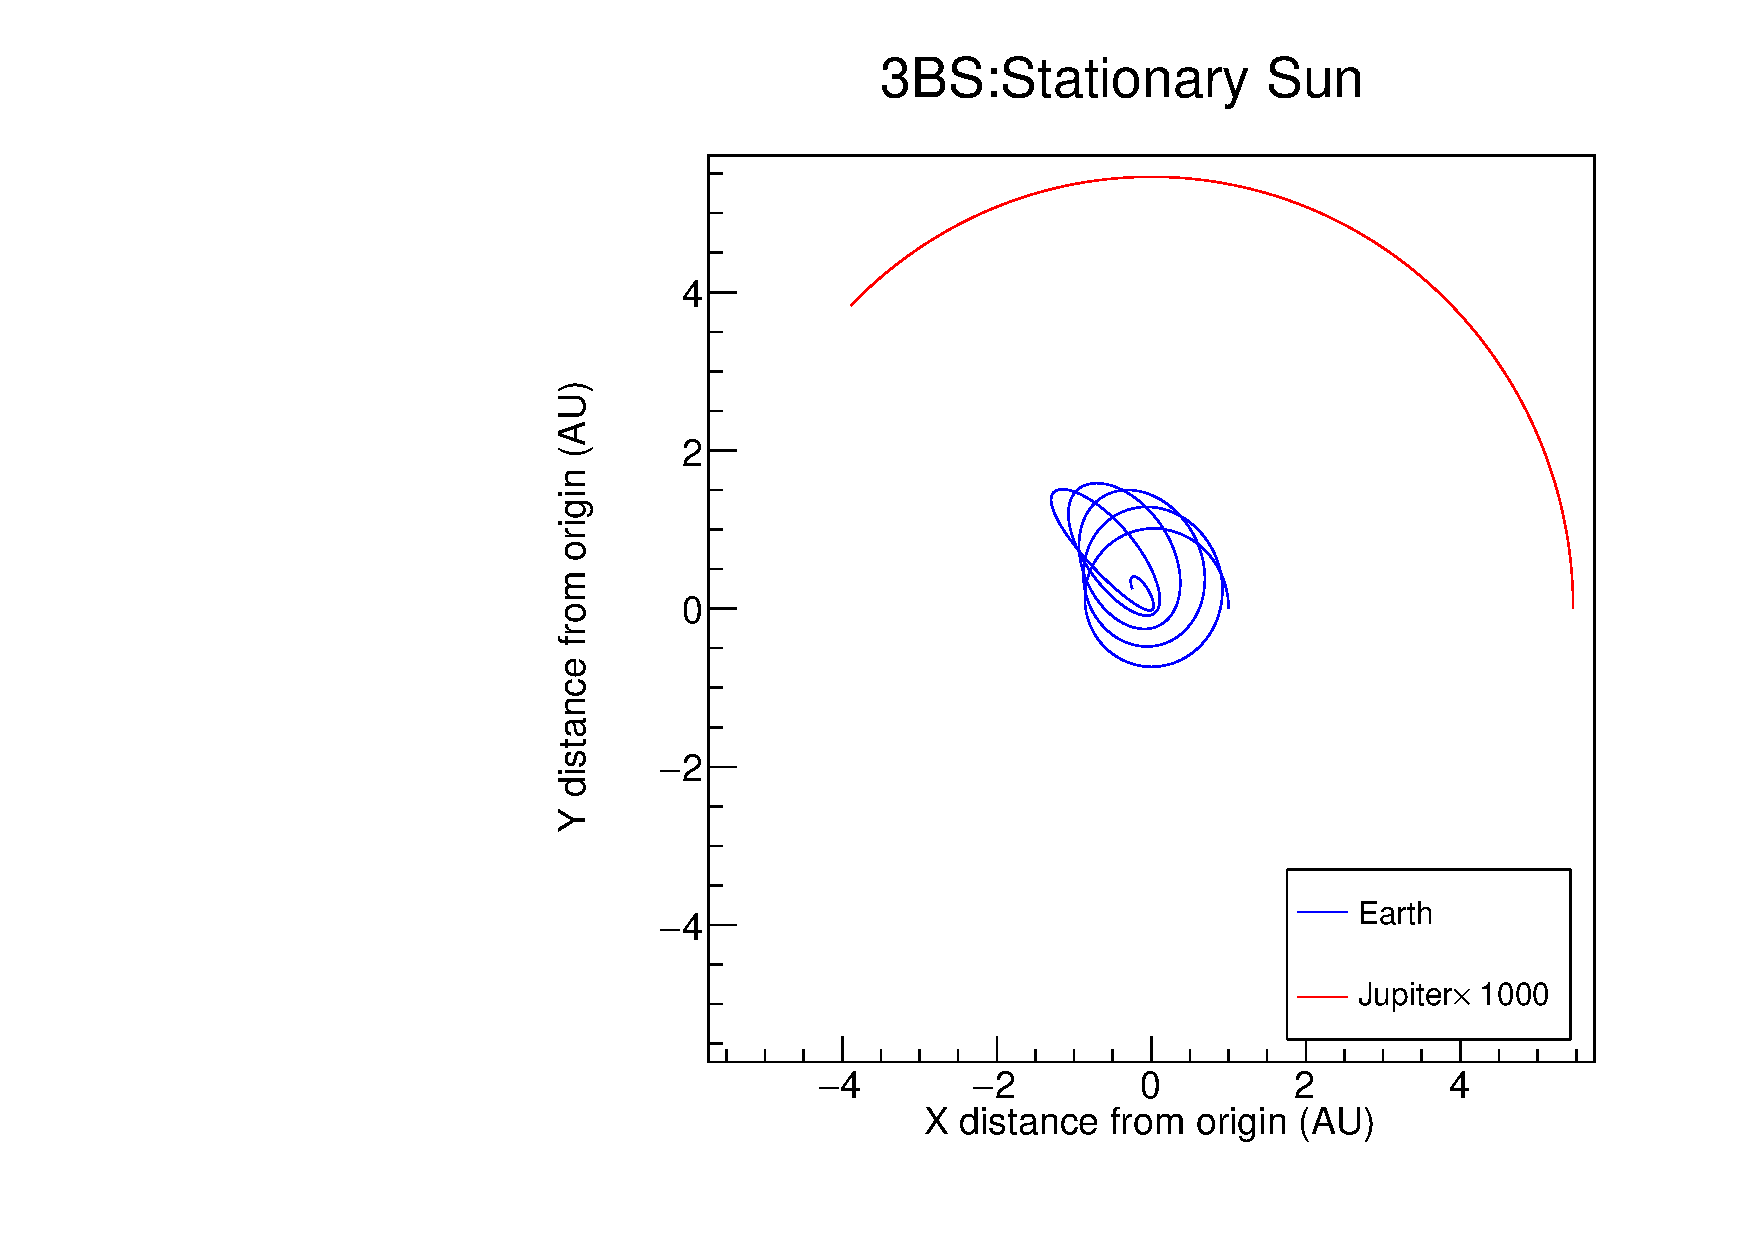
\includegraphics[width=0.5\textwidth]{ESJFVerlet_x1000.pdf}
  \caption{Plot of 3 body system with Earth, Jupiter, and a stationary sun using $\times 1000$ Jupiter mass. Used a shorter timespan because this heavy Jupiter causes Earth to ``hit the sun'', then go barreling out many AU so the orbital structure is no longer visible. Time interval: 4.8 years, Time steps: 13000, Algorithm: Verlet.}
  \label{fig:ESJFVerlet_x1000}
 \end{figure}
 
 \chapter{All Major Solar System Bodies: Plots}
   \begin{SCfigure}
 \centering
   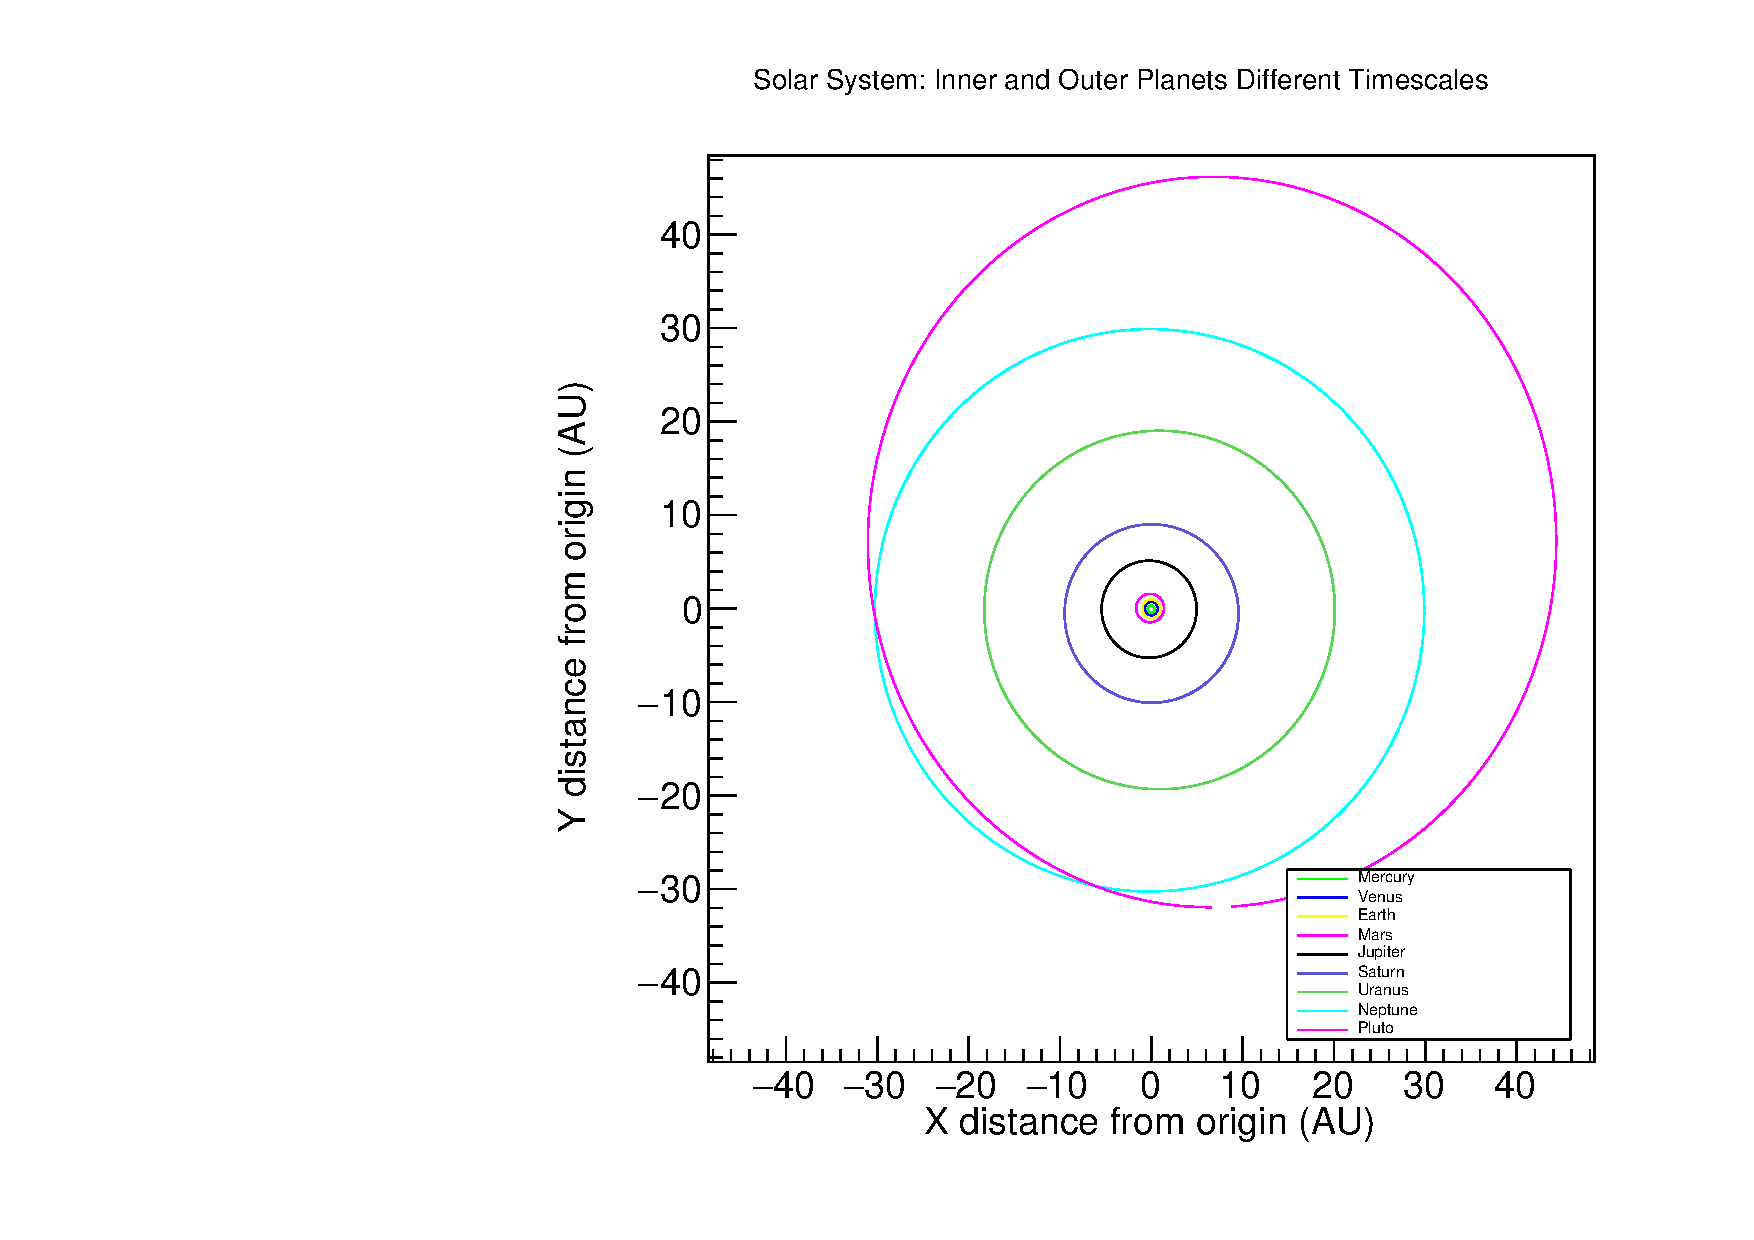
\includegraphics[width=0.5\textwidth]{all_bodies_inner_outer_sep_Verlet.pdf}
  \caption{Plot of all major bodies with inner and outer planets calculated separately. Inner Planets - Time: 5 years, Time Steps: 5000, Algorithm: Verlet. Outer Planets - Time: 250 years, Time Steps: 25000, Algorithm: Verlet}
  \label{fig:all_bodies_inner_outer_sep_Verlet}
 \end{SCfigure}

 \begin{SCfigure}
 \centering
   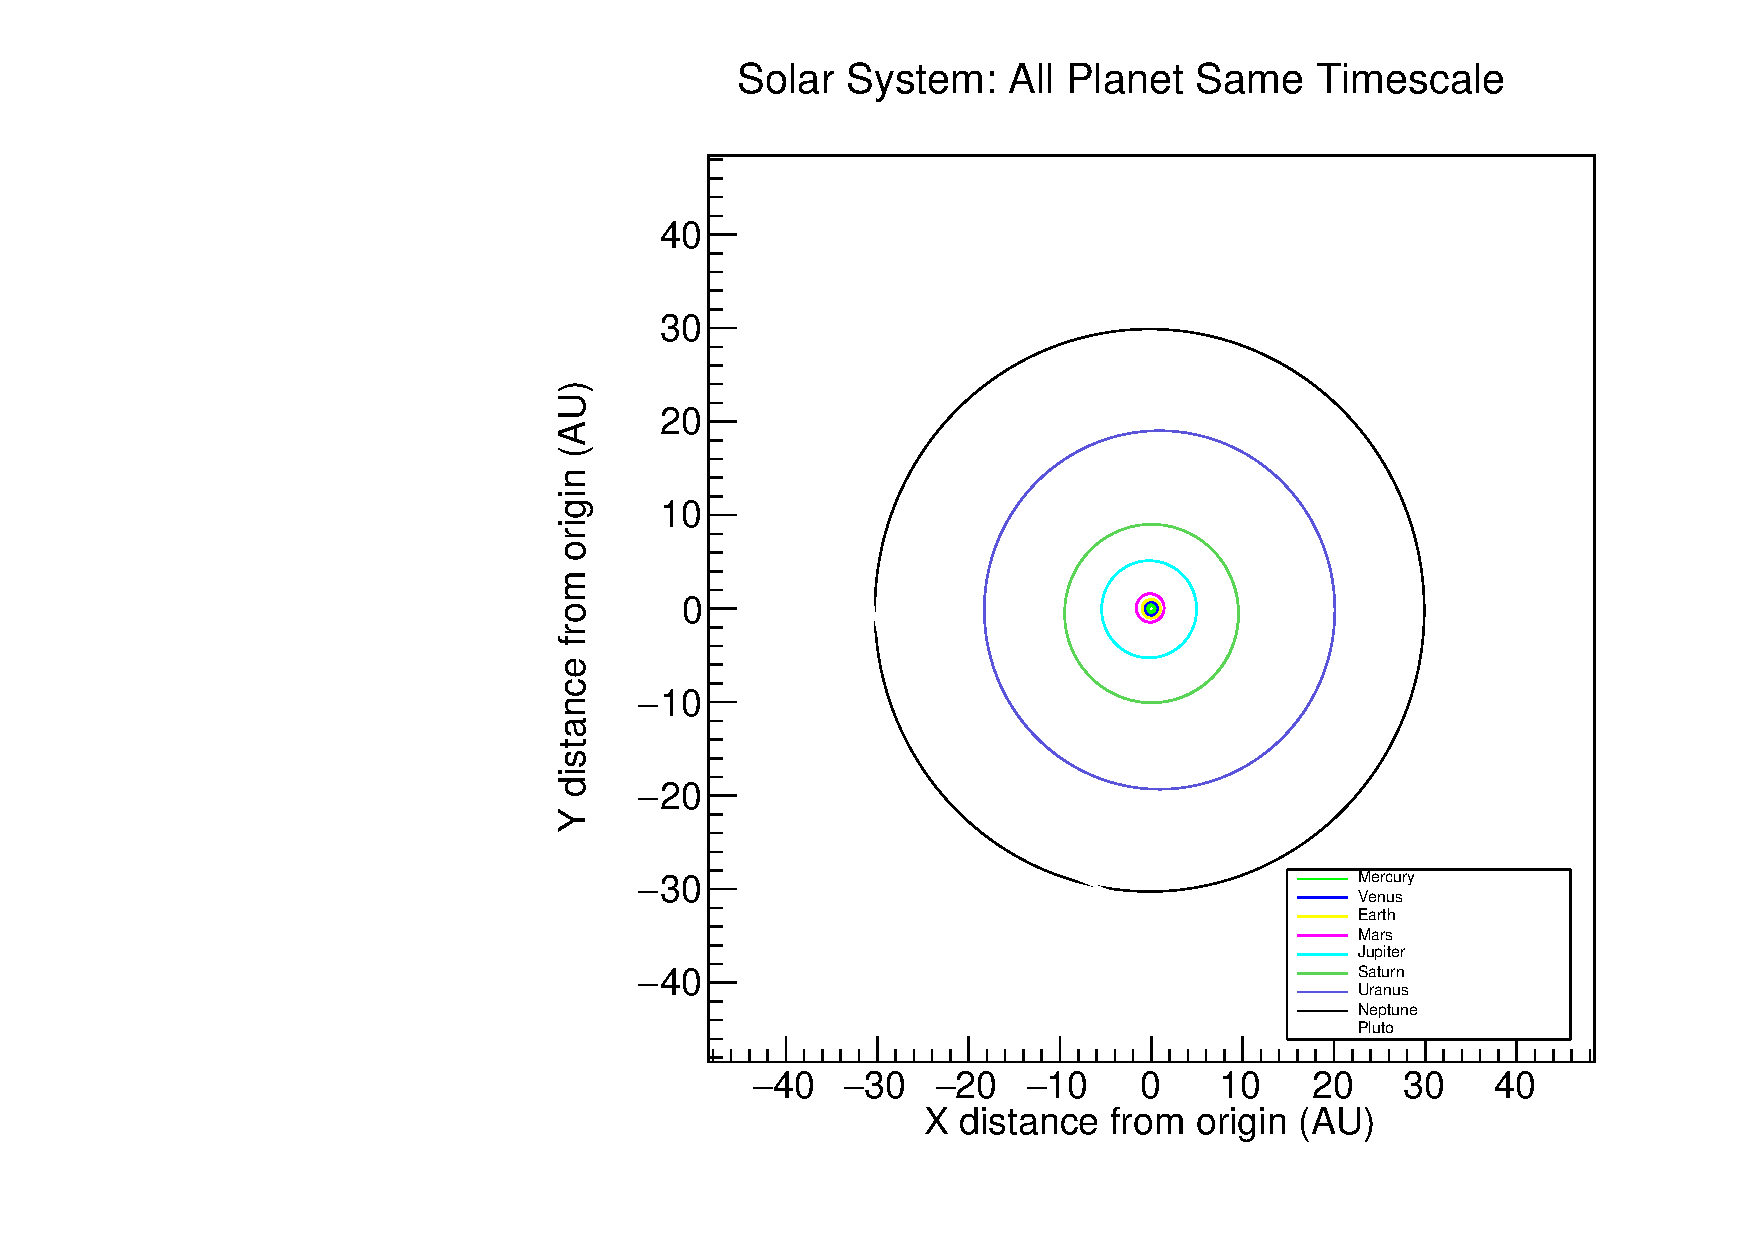
\includegraphics[width=0.5\textwidth]{all_bodies_same_time_Verlet.pdf}
  \caption{Plot of all major bodies calculated at the same time. Time: 250 years, Time Steps: 25000, Algorithm: Verlet}
  \label{fig:all_bodies_same_time_Verlet}
 \end{SCfigure}
 
  \begin{SCfigure}
 \centering
   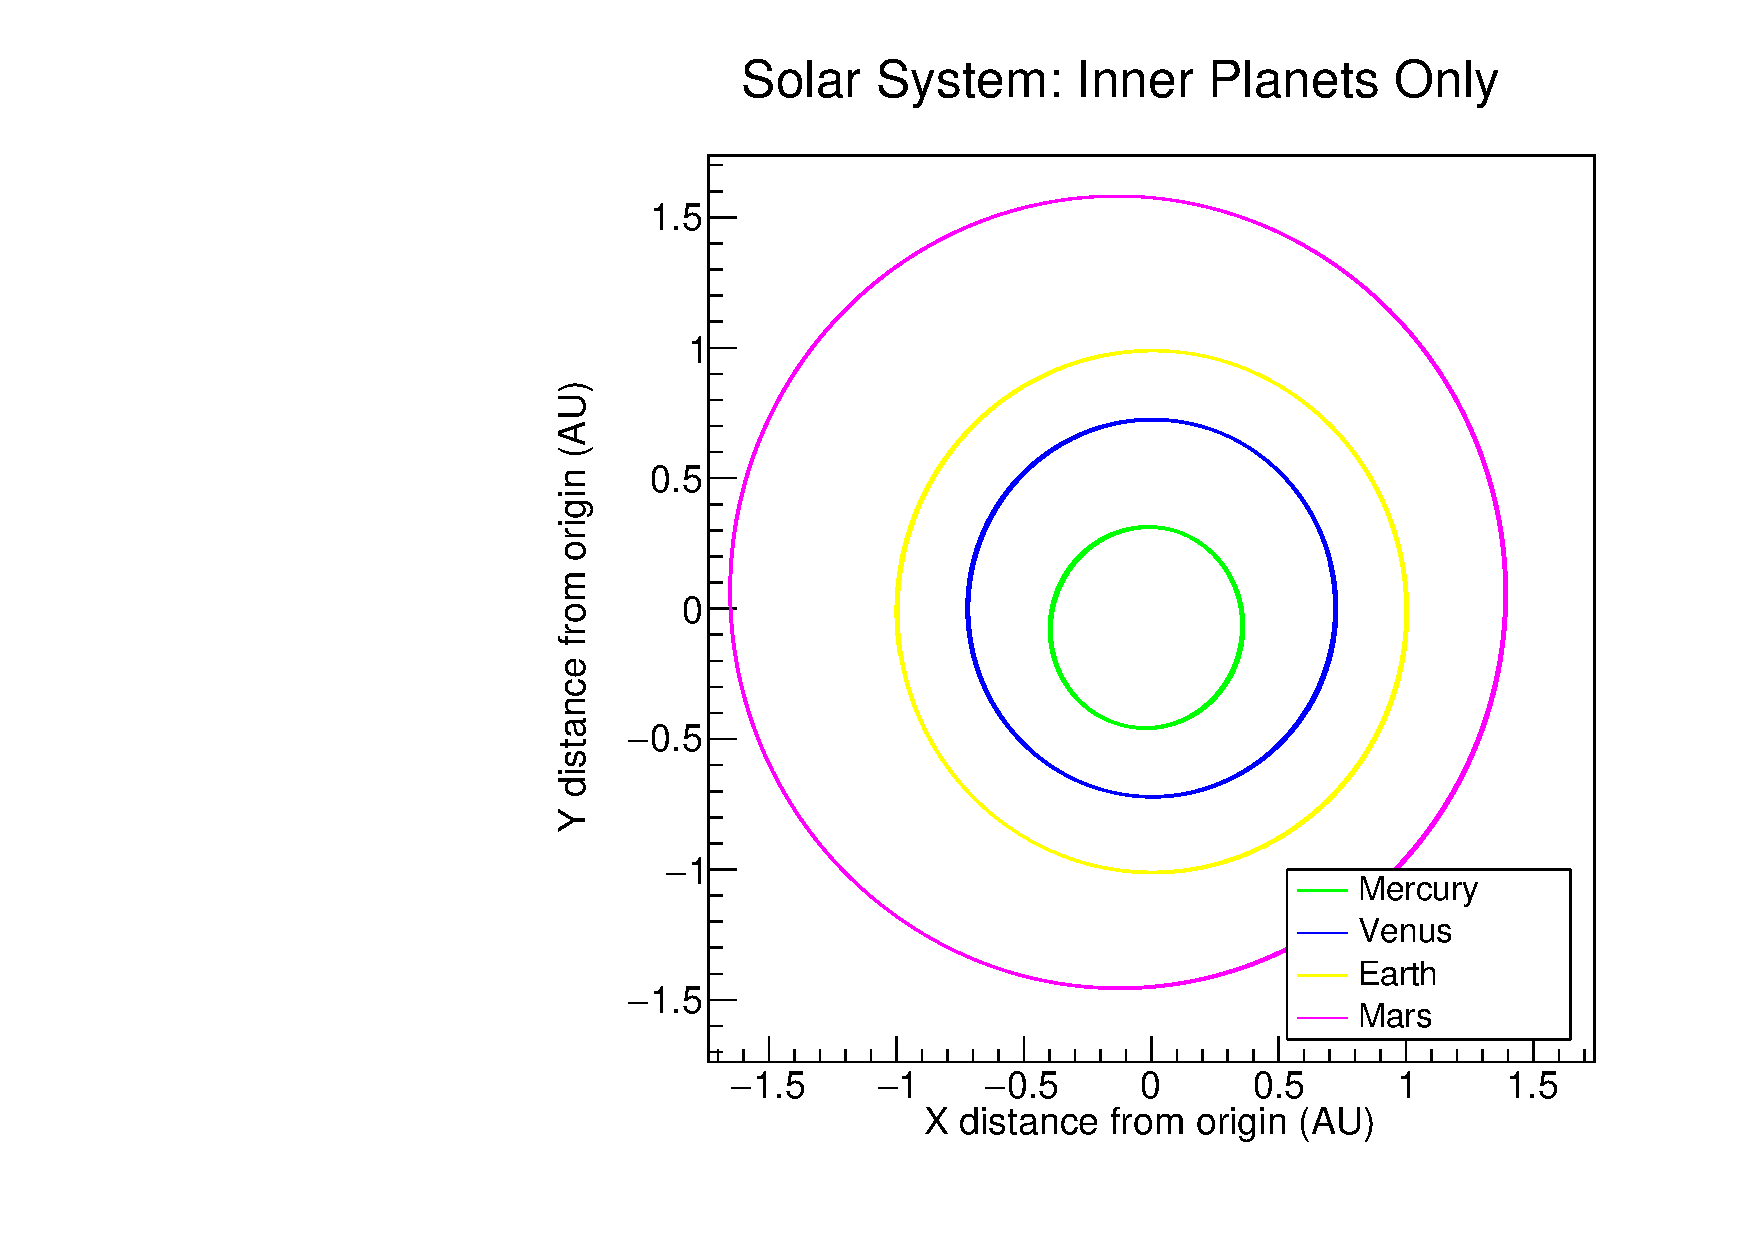
\includegraphics[width=0.5\textwidth]{inner_only_RK4.pdf}
  \caption{Inner solar system. Time: 5 years, Time Steps: 5000, Algorithm: RK4}
  \label{fig:inner_only_RK4}
 \end{SCfigure}
 
   \begin{SCfigure}
 \centering
   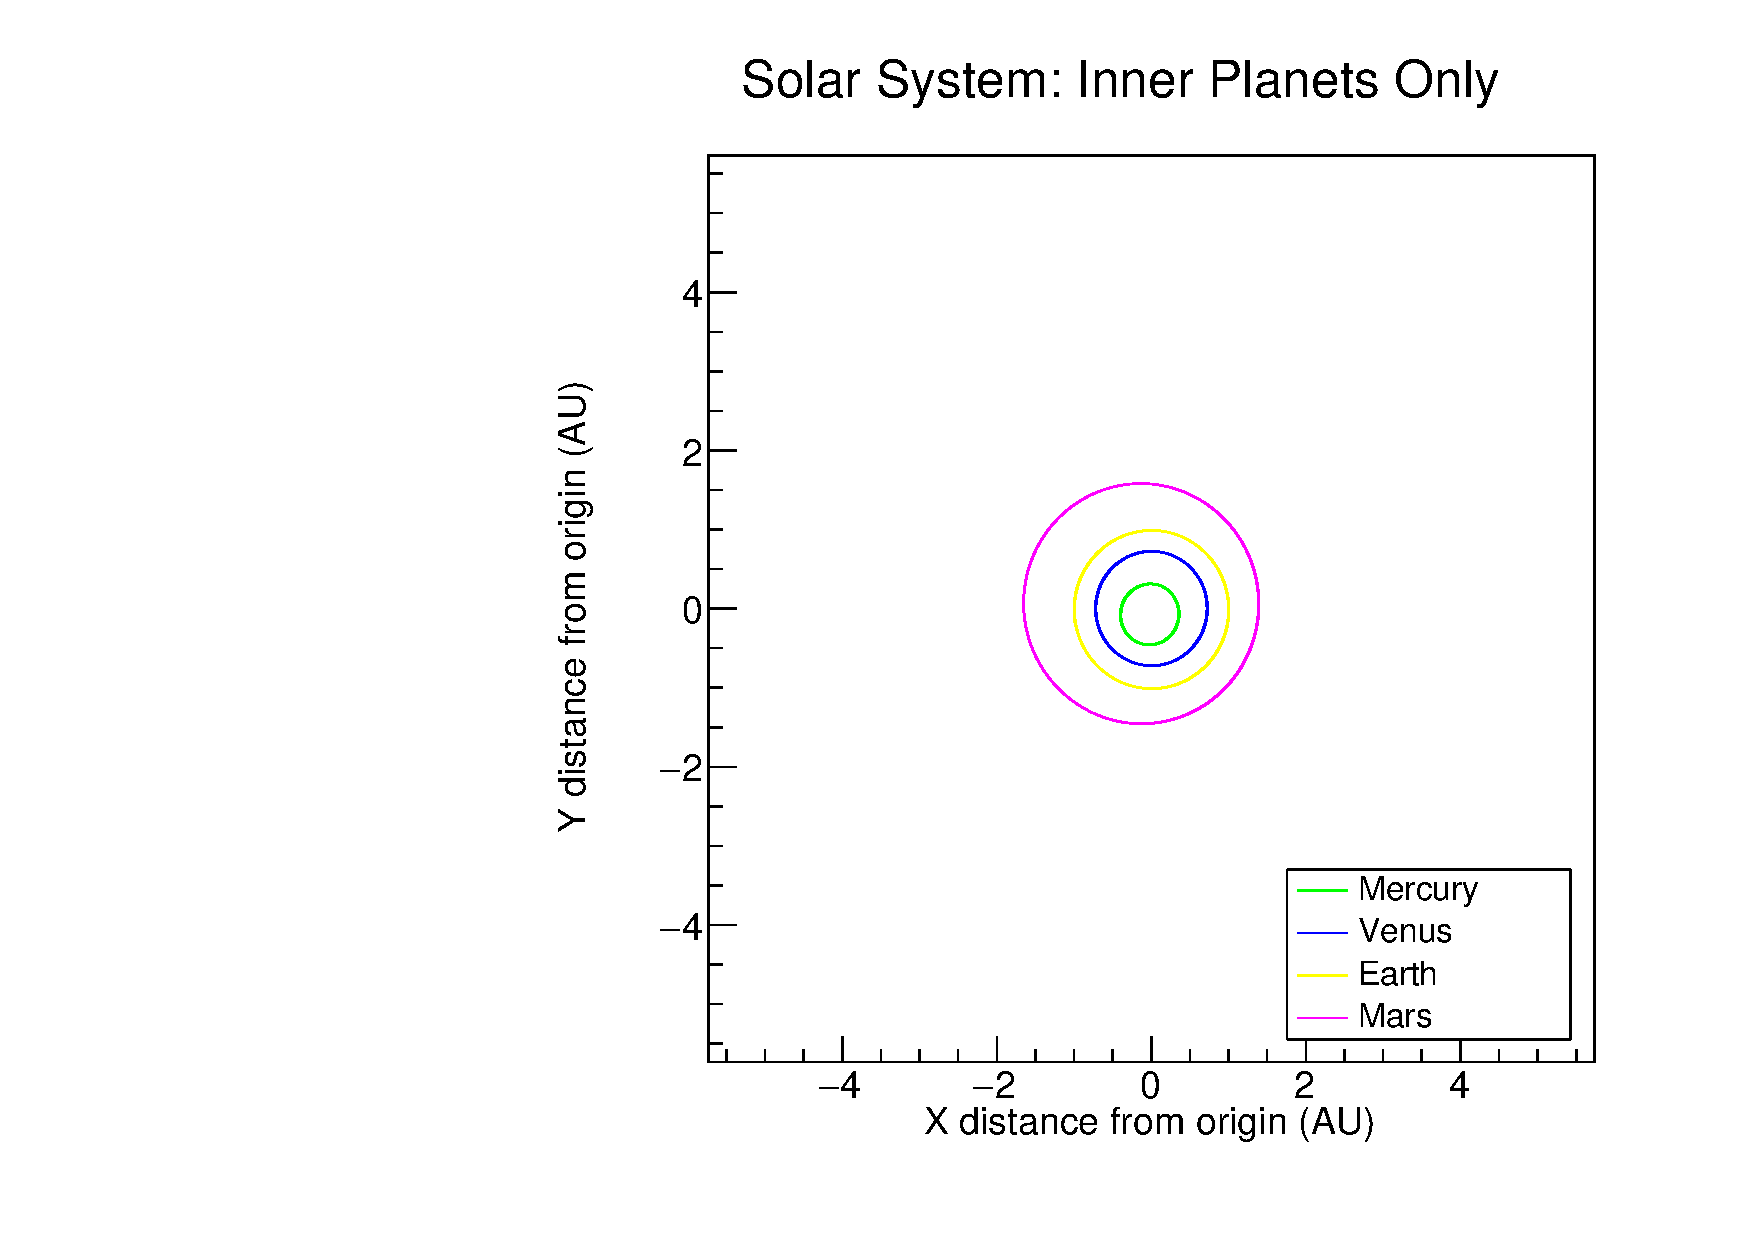
\includegraphics[width=0.5\textwidth]{inner_only_Verlet.pdf}
  \caption{Inner solar system. Time: 5 years, Time Steps: 5000, Algorithm: Verlet}
  \label{fig:inner_only_Verlet}
 \end{SCfigure}
 
  \begin{SCfigure}
 \centering
   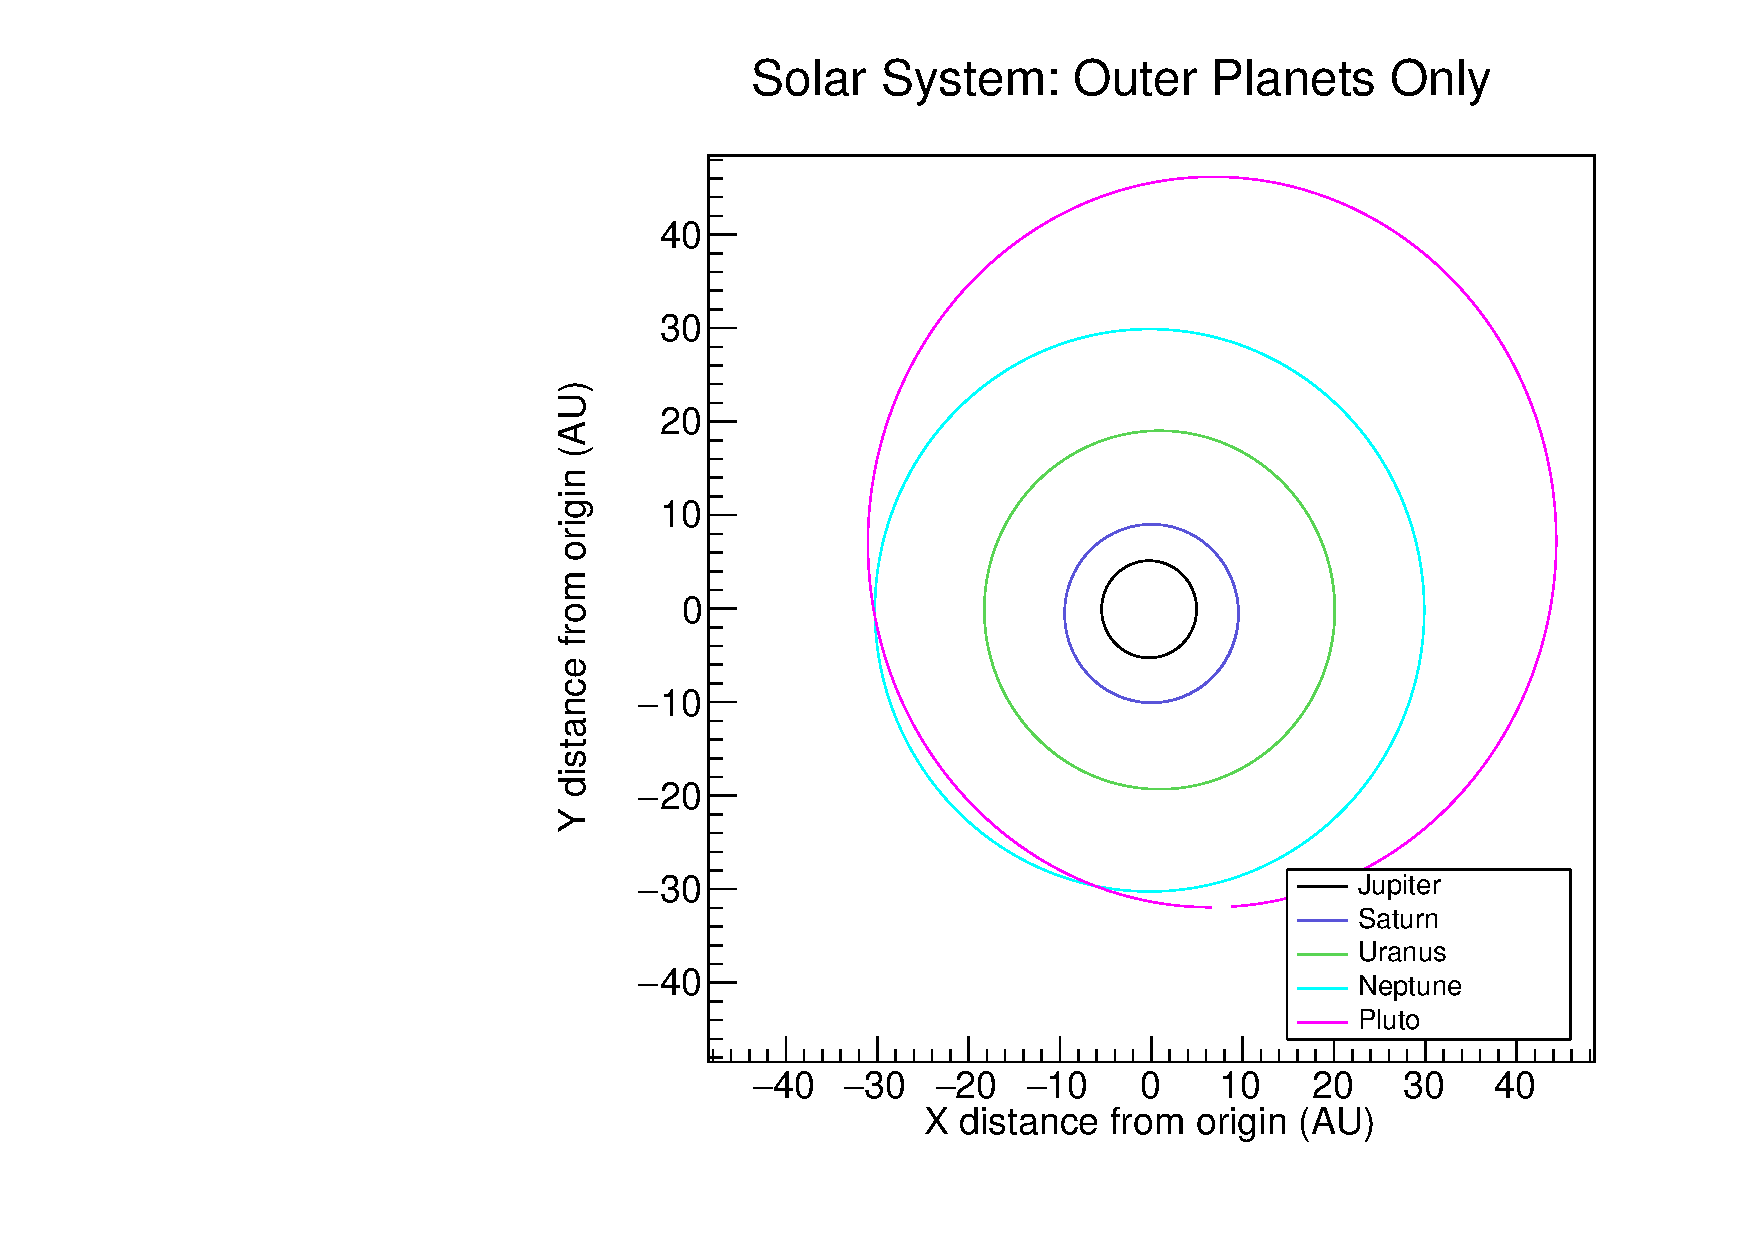
\includegraphics[width=0.5\textwidth]{outer_only_RK4.pdf}
  \caption{Outer solar system. Time: 250 years, Time Steps: 25000, Algorithm: RK4}
  \label{fig:outer_only_RK4}
 \end{SCfigure}
 
   \begin{SCfigure}
 \centering
   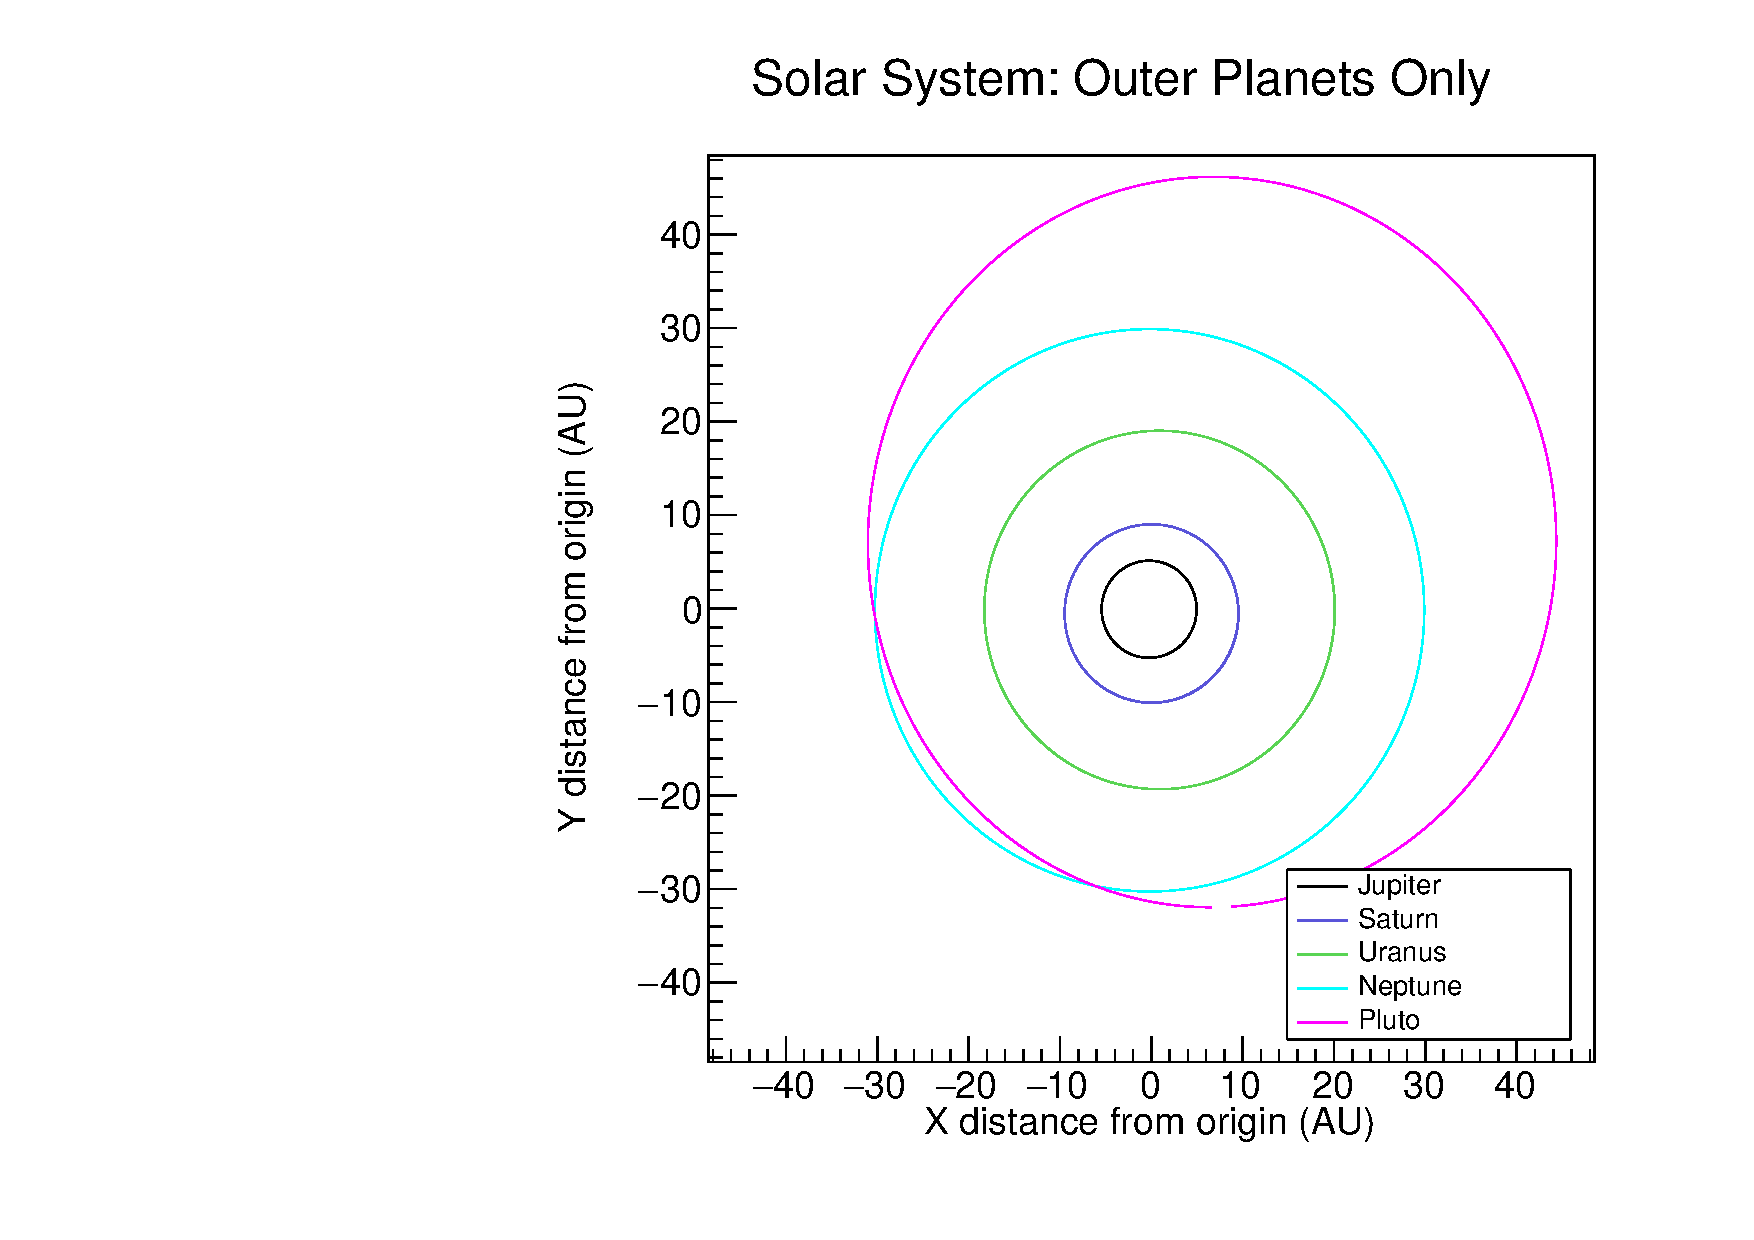
\includegraphics[width=0.5\textwidth]{outer_only_Verlet.pdf}
  \caption{Outer solar system. Time: 250 years, Time Steps: 25000, Algorithm: Verlet}
  \label{fig:outer_only_Verlet}
 \end{SCfigure}
 
 \chapter{All RK4 Code}\label{app:rk4}
 \singlespacing
 \begin{Verbatim}[fontsize=\small]
void SolarSystem::RK4(){
  _solved = true;
  double Fx,Fy,Fz;

  for( int i = 1; i <= _Ntime; i++ ){
    vector< vector< double > > k1, k2, k3; 
    for( unsigned int iPlanet = 0; iPlanet < GetN(); iPlanet++ ){

      // Keep planet in same position if it is fixed
      if(_vPlanets.at(iPlanet).Fixed()){
	_vPlanets.at(iPlanet).AddCoordinates(i*_step,
					     _vPlanets.at(iPlanet).X(i-1),
					     _vPlanets.at(iPlanet).Y(i-1),
					     _vPlanets.at(iPlanet).Z(i-1),
					     _vPlanets.at(iPlanet).Vx(i-1),
					     _vPlanets.at(iPlanet).Vy(i-1),
					     _vPlanets.at(iPlanet).Vz(i-1));				    
	vector<double> placeholder;
	k1.push_back(placeholder);
      }
      else{

	// calculate k1
	vector<double> k1i;
	k1i.push_back( _step*_vPlanets.at(iPlanet).Vx(i-1) );
	k1i.push_back( _step*_vPlanets.at(iPlanet).Vy(i-1) );
	k1i.push_back( _step*_vPlanets.at(iPlanet).Vz(i-1) );

	TotalForce(iPlanet,i-1,Fx,Fy,Fz);
	k1i.push_back( _step*Fx/_vPlanets.at(iPlanet).M() );
	k1i.push_back( _step*Fy/_vPlanets.at(iPlanet).M() );
	k1i.push_back( _step*Fz/_vPlanets.at(iPlanet).M() );

	// Advance f(t_i,y_i)->f(t_i+h/2,y_i+k1/2)
	_vPlanets.at(iPlanet).AddCoordinates(i*_step,
					     _vPlanets.at(iPlanet).X(i-1)+k1i.at(0)/2.,
					     _vPlanets.at(iPlanet).Y(i-1)+k1i.at(1)/2.,
					     _vPlanets.at(iPlanet).Z(i-1)+k1i.at(2)/2.,
					     _vPlanets.at(iPlanet).Vx(i-1)+k1i.at(3)/2.,
					     _vPlanets.at(iPlanet).Vy(i-1)+k1i.at(4)/2.,
					     _vPlanets.at(iPlanet).Vz(i-1)+k1i.at(5)/2.);
	k1.push_back(k1i);
      }
    }
    
    for( unsigned int iPlanet = 0; iPlanet < GetN(); iPlanet++ ){
      if(_vPlanets.at(iPlanet).Fixed()){
	vector<double> placeholder;
	k2.push_back(placeholder);
      }
      else{
	// calculate k2
	vector<double> k2i;
	k2i.push_back( _step*_vPlanets.at(iPlanet).Vx(i));
	k2i.push_back( _step*_vPlanets.at(iPlanet).Vy(i));
	k2i.push_back( _step*_vPlanets.at(iPlanet).Vz(i));

	TotalForce(iPlanet,i,Fx,Fy,Fz);
	k2i.push_back( _step*Fx/_vPlanets.at(iPlanet).M() );
	k2i.push_back( _step*Fy/_vPlanets.at(iPlanet).M() );
	k2i.push_back( _step*Fz/_vPlanets.at(iPlanet).M() );

	// Advance f(t_i+h/2,y_i+k1/2)->f(t_i+h/2,y_i+k2/2)
	_vPlanets.at(iPlanet).SetX(_vPlanets.at(iPlanet).X(i-1)+k2i.at(0)/2.,i);
	_vPlanets.at(iPlanet).SetY(_vPlanets.at(iPlanet).Y(i-1)+k2i.at(1)/2.,i);
	_vPlanets.at(iPlanet).SetZ(_vPlanets.at(iPlanet).Z(i-1)+k2i.at(2)/2.,i);
	_vPlanets.at(iPlanet).SetVx(_vPlanets.at(iPlanet).Vx(i-1)+k2i.at(3)/2.,i);
	_vPlanets.at(iPlanet).SetVy(_vPlanets.at(iPlanet).Vy(i-1)+k2i.at(4)/2.,i);
	_vPlanets.at(iPlanet).SetVz(_vPlanets.at(iPlanet).Vz(i-1)+k2i.at(5)/2.,i);
	k2.push_back(k2i);
      }
    }
  
    for( unsigned int iPlanet = 0; iPlanet < GetN(); iPlanet++ ){
      if(_vPlanets.at(iPlanet).Fixed()){
	vector<double> placeholder;
	k3.push_back(placeholder);
      }
      else{
	// calculate k3
	vector<double> k3i;
	k3i.push_back( _step*_vPlanets.at(iPlanet).Vx(i));
	k3i.push_back( _step*_vPlanets.at(iPlanet).Vy(i));
	k3i.push_back( _step*_vPlanets.at(iPlanet).Vz(i));

	TotalForce(iPlanet,i,Fx,Fy,Fz);
	k3i.push_back( _step*Fx/_vPlanets.at(iPlanet).M() );
	k3i.push_back( _step*Fy/_vPlanets.at(iPlanet).M() );
	k3i.push_back( _step*Fz/_vPlanets.at(iPlanet).M() );

	// Advance f(t_i+h/2,y_i+k2/2)->f(t_i+h,y_i+k3)
	_vPlanets.at(iPlanet).SetX(_vPlanets.at(iPlanet).X(i-1)+k3i.at(0),i);
	_vPlanets.at(iPlanet).SetY(_vPlanets.at(iPlanet).Y(i-1)+k3i.at(1),i);
	_vPlanets.at(iPlanet).SetZ(_vPlanets.at(iPlanet).Z(i-1)+k3i.at(2),i);
	_vPlanets.at(iPlanet).SetVx(_vPlanets.at(iPlanet).Vx(i-1)+k3i.at(3),i);
	_vPlanets.at(iPlanet).SetVy(_vPlanets.at(iPlanet).Vy(i-1)+k3i.at(4),i);
	_vPlanets.at(iPlanet).SetVz(_vPlanets.at(iPlanet).Vz(i-1)+k3i.at(5),i);
	k3.push_back(k3i);
      }
    }

    for( unsigned int iPlanet = 0; iPlanet < GetN(); iPlanet++ ){
      if(!_vPlanets.at(iPlanet).Fixed()){
	// calculate k4
	vector<double> k4i;
	k4i.push_back( _step*_vPlanets.at(iPlanet).Vx(i));
	k4i.push_back( _step*_vPlanets.at(iPlanet).Vy(i));
	k4i.push_back( _step*_vPlanets.at(iPlanet).Vz(i));

	Fx = Fy = Fz = 0.;
	TotalForce(iPlanet,i,Fx,Fy,Fz);
	k4i.push_back( _step*Fx/_vPlanets.at(iPlanet).M() );
	k4i.push_back( _step*Fy/_vPlanets.at(iPlanet).M() );
	k4i.push_back( _step*Fz/_vPlanets.at(iPlanet).M() );

	// Advance y_(i+1) = y_i + (1/6)(k1+2k2+2k3+k4)
	_vPlanets.at(iPlanet).SetX(_vPlanets.at(iPlanet).X(i-1)
				   +(k1.at(iPlanet).at(0)
				   +2.*k2.at(iPlanet).at(0)
				   +2.*k3.at(iPlanet).at(0)
				     +k4i.at(0))/6.,i);
	_vPlanets.at(iPlanet).SetY(_vPlanets.at(iPlanet).Y(i-1)
				   +(k1.at(iPlanet).at(1)
				   +2.*k2.at(iPlanet).at(1)
				   +2.*k3.at(iPlanet).at(1)
				     +k4i.at(1))/6.,i);
	_vPlanets.at(iPlanet).SetZ(_vPlanets.at(iPlanet).Z(i-1)
				   +(k1.at(iPlanet).at(2)
				   +2.*k2.at(iPlanet).at(2)
				   +2.*k3.at(iPlanet).at(2)
				     +k4i.at(2))/6.,i);
	_vPlanets.at(iPlanet).SetVx(_vPlanets.at(iPlanet).Vx(i-1)
				    +(k1.at(iPlanet).at(3)
				    +2.*k2.at(iPlanet).at(3)
				    +2.*k3.at(iPlanet).at(3)
				      +k4i.at(3))/6.,i);
	_vPlanets.at(iPlanet).SetVy(_vPlanets.at(iPlanet).Vy(i-1)
				    +(k1.at(iPlanet).at(4)
				    +2.*k2.at(iPlanet).at(4)
				    +2.*k3.at(iPlanet).at(4)
				      +k4i.at(4))/6.,i);
	_vPlanets.at(iPlanet).SetVz(_vPlanets.at(iPlanet).Vz(i-1)
				    +(k1.at(iPlanet).at(5)
				    +2.*k2.at(iPlanet).at(5)
				    +2.*k3.at(iPlanet).at(5)
				      +k4i.at(5))/6.,i);
      }
    }
  }
}
 \end{Verbatim}
 \doublespacing
 
\nocite{*}
\bibliographystyle{plain}
\bibliography{ReportProject3.bib}
\end{document}          
